% APMA 4302 final report — parallel Monte Carlo + PETSc PDE / Krylov course bridge
% Compile from this directory: pdflatex main.tex (twice for stable refs)
\documentclass[11pt]{article}
\usepackage[margin=1in]{geometry}
\usepackage{graphicx}
\usepackage{subcaption}
\usepackage{amsmath,amssymb}
\usepackage{booktabs}
\usepackage{hyperref}
\usepackage{caption}
\usepackage{enumitem}
\usepackage{parskip}
\setlength{\parskip}{0.55em}
\captionsetup{font=footnotesize,skip=5pt,width=0.92\linewidth}
% Compact figures: stay near prose, smaller than full text width
\newcommand{\figw}{0.52\textwidth}
\newcommand{\figwp}{0.44\textwidth}

\graphicspath{{figures/}}

\title{\textbf{Parallel Monte Carlo Option Pricing with PETSc:}\\
HPC reductions, calibrated volatility, and PETSc PDE / Krylov demos}
\author{APMA 4302 --- Columbia University\\
\small (Daniel David / UNI: dad2232)}
\date{\today}

\begin{document}
\maketitle

\begin{abstract}
This report documents a deliberately \textbf{broad} scientific computing project that
ties together three threads normally taught as separate weeks in a PETSc-aware
numerical methods / HPC curriculum: \textbf{(i)} scalable Monte Carlo estimation with
rigorous uncertainty quantification, \textbf{(ii)} sparse linear algebra and
preconditioned Krylov solvers on representative PDE discretizations, and
\textbf{(iii)} reproducible visualization of fields and trajectories through
ParaView. The financial thread prices European, Asian, and barrier-style options
under geometric Brownian motion (GBM) using MPI-parallel path batches and global
reductions implemented with PETSc's programming model~\cite{petsc-user-ref,petsc-efficient}.
The PDE thread follows the \emph{matrix--vector--solver} pedagogy of Bueler's SIAM
text~\cite{bueler2020petsc}: Poisson on structured grids, implicit heat and
advection--diffusion time steps, and small diagnostic sweeps over \textsf{KSP} and
\textsf{PC} choices. A scalar \textbf{SNES} solve recovers implied volatility from
Black--Scholes as a clean nonlinear equation example. \textbf{Phase~2} connects the
same Monte Carlo engine to \textbf{historical SPY data}: rolling realized volatility
replaces a toy constant $\sigma$, and a roll-forward experiment reprices an
ATM-style call along a sparse calendar of market snapshots.

\medskip
\noindent\textbf{Primary aim.}
The goal of this project was \emph{neither} finance \emph{nor} PDE theory for their own
sake: those threads are \textbf{vehicles} for practicing a single style of work at
scale---\textbf{PETSc + MPI} programming with partitioned data, global reductions,
solver objects, and honestly reported timings. Monte Carlo paths and grid-based PDE
steps simply expose \emph{different} dominant costs (sampling vs.\ sparse linear
algebra) while demanding the \emph{same} engineering habits: isolate the numerical
kernel, parallelize cleanly, and validate with layered evidence (closed forms, mesh
refinement, statistical error decay, and performance curves)~\cite{bueler2020petsc,petsc-user-ref}.
That unification is what large-scale scientific computing increasingly expects from
practitioners who must move between kernels without reinventing their software stack
each time~\cite{petsc-efficient}.

\medskip
\noindent\textbf{Citations in one line.}
Options theory follows Black--Scholes and Merton~\cite{blackscholes,merton1973};
PETSc software practice follows Balay et al.~\cite{petsc-user-ref,petsc-efficient};
PDE discretization + Krylov/Newton intuition follows Bueler~\cite{bueler2020petsc};
visualization practice follows Ahrens et al.~\cite{paraview-guide}.
\end{abstract}

\tableofcontents
\newpage

\section{Introduction: problem, audience, and claims}

\subsection{The motivating tension}
Monte Carlo (MC) option pricing is attractive because it scales gracefully in the
number of paths and because it extends to payoffs where closed forms are awkward
(e.g.\ path-dependent Asian averages and barrier knock-out structures). Yet MC is
not ``free parallelism'': one still needs deterministic reproducibility policies,
stable variance estimators, and careful interpretation of parallel timings when
collectives and load imbalance enter the story.

At the same time, a PETSc-centered numerical methods course emphasizes different
bottlenecks: sparse matrix assembly, preconditioned Krylov iterations, and nonlinear
solvers~\cite{bueler2020petsc}. Those kernels look different from MC on the surface,
but they share a common engineering spine: \textbf{partition data, compute locally,
reduce globally, measure time and iteration counts honestly}~\cite{petsc-efficient}.

\subsection{What we claim this repository demonstrates}
We claim three \textbf{research-grade} outcomes supported by artifacts in the report
figures and CSV logs:
\begin{enumerate}[leftmargin=*]
  \item \textbf{Statistical correctness and scaling of the MC pricer:} European
  prices match Black--Scholes at tolerances consistent with standard error budgets;
  error vs.\ $N$ follows the expected square-root law on log--log plots; barrier
  sweeps show how payoff geometry modulates variance; strong/weak scaling curves
  document parallel behavior for a fixed implementation.
  \item \textbf{Deterministic PDE pipeline correctness and solver literacy:} Poisson
  spatial convergence under mesh refinement is consistent with finite-difference
  expectations; PC and KSP sweeps make preconditioner and outer-solver tradeoffs
  visible on the same discrete operator; heat and advection--diffusion ParaView
  exports document time-evolving fields consistent with implicit stepping, and
  trajectory \texttt{.vtp} bundles connect the Monte Carlo thread to the same
  visualization discipline~\cite{paraview-guide}.
  \item \textbf{Phase~2 realism:} realized volatility from historical SPY data is
  materially time-varying; roll-forward repricing shows how the \emph{same} MC
  engine responds when inputs drift with the market rather than remaining stylized
  constants.
\end{enumerate}

\subsection{Where the ideas came from (intellectual lineage)}
The \textbf{financial modeling} layer is textbook GBM risk-neutral pricing as
presented in foundational derivatives references~\cite{blackscholes,merton1973}.
The \textbf{PETSc object model} (Vec, Mat, KSP, PC, SNES) and the habit of treating
performance as a first-class output follow the PETSc team's user manual and the
original PETSc software paper~\cite{petsc-user-ref,petsc-efficient}. The
\textbf{PDE discretization + Krylov + Newton} narrative is intentionally aligned with
Bueler's \emph{PETSc for Partial Differential Equations}~\cite{bueler2020petsc},
because that book is written precisely for readers who need to connect mathematical
definitions to working code: structured grids, residual-based stopping, and
preconditioner choices that are not black boxes.

The \textbf{visualization} layer follows standard ParaView practice for scientific
vector/tensor data~\cite{paraview-guide}. The project-specific runbook is
\textbf{Appendix A} of \texttt{PROJECT\_OUTLINE.md} in the repository (legacy filename
\texttt{PARAVIEW\_GUIDE\_PETSC.md} redirects there); it documents how \texttt{.pvd} time
collections and \texttt{.vtp} surface snapshots were produced from PETSc fields.

\section{Mathematical models}
\subsection{Option pricing under GBM}
Under risk-neutral GBM,
\[
  dS_t = r S_t\,dt + \sigma S_t\,dW_t,
\]
with an exact exponential integrator over $\Delta t$ for path simulation, as is
standard in Monte Carlo implementations~\cite{blackscholes,merton1973}. Payoffs
implemented in the codebase include European calls, Asian averages, and barrier
knock-out structures; these choices stress different variance profiles and
different parallel workload shapes (e.g.\ barrier paths may terminate early in
alternative implementations; here the emphasis is on statistical behavior vs.\
barrier level sweeps).

\subsection{Representative PDEs (PETSc demos)}
Poisson (elliptic), heat (parabolic), and linear advection--diffusion models follow
the formulations and discretization narrative in Bueler~\cite{bueler2020petsc}:
\begin{align*}
  -\Delta u &= f \quad \text{(Poisson)},\\
  u_t - \kappa \Delta u &= g \quad \text{(heat)},\\
  u_t + \mathbf{v}\!\cdot\!\nabla u - \nu \Delta u &= s \quad \text{(advection--diffusion)}.
\end{align*}
These are not ``toy unrelated PDEs'': they are the canonical PDE classes used to
introduce FD stencils, stability of implicit time stepping, and the nonsymmetric
shifts induced by advection operators---exactly the vocabulary Bueler uses to build
toward realistic PETSc workflows~\cite{bueler2020petsc}.

\section{Numerical methods and PETSc objects}
\subsection{Finite differences and Krylov solvers}
We use structured five-point Laplacians on the unit square for Poisson, consistent
with a first-course finite-difference treatment~\cite{bueler2020petsc}. Linear
systems are solved with PETSc \textsf{KSP} + \textsf{PC}. For SPD Poisson-like
operators, CG with Jacobi is a transparent baseline that exposes iteration counts
and residual norms without hiding complexity inside a factorization black
box~\cite{bueler2020petsc,petsc-user-ref}.

\paragraph{Advection--diffusion in parallel.}
For parallel runs, incomplete LU as a preconditioner is often unavailable or
fragile for distributed sparse matrices; our advection--diffusion driver therefore
defaults to \textbf{CG + Jacobi} for the implicit step (GMRES + Jacobi is a common
alternative when nonsymmetry is more pronounced). This is not merely an
implementation detail: it is the same ``preconditioners are not magic'' lesson
emphasized in Krylov coursework and in Bueler's treatment of scalable
preconditioning~\cite{bueler2020petsc,petsc-user-ref}.

\subsection{Nonlinear solve (SNES) for implied volatility}
We recover implied $\sigma$ from a synthetic market price by solving the scalar
equation $\mathrm{BS}(\sigma)=V_{\mathrm{mkt}}$ with PETSc \textsf{SNES},
optionally supplying a hand-coded $1\times 1$ Jacobian (vega). This is a deliberate
bridge to the Newton / SNES week: the problem is tiny, but the software pattern is
the same as large residual equations~\cite{bueler2020petsc,petsc-user-ref}.

\section{Parallel Monte Carlo engine: what was built and how we read the evidence}
\subsection{Implementation narrative}
The Monte Carlo engine partitions path indices across MPI ranks, simulates GBM paths
(including optional antithetic pairing for variance reduction), evaluates payoffs,
and performs global reductions for the mean, mean-square contributions needed for
variance, and valid path counts. This is the same SPMD structure PETSc users apply
to partitioned meshes, except the ``mesh cells'' are replaced by path
batches~\cite{petsc-efficient}.

\subsection{Interpreted results (Monte Carlo)}
\textbf{Verification.} European MC prices align with Black--Scholes within
uncertainty budgets implied by the standard error; this is the first sanity check
that parallel RNG partitioning and reductions are consistent~\cite{blackscholes}.

\textbf{Convergence in $N$.} Log--log plots of error vs.\ $N$ are the correct
statistical diagnostic: we do not expect machine-precision convergence, but we do
expect the error to shrink with the inverse square root of independent samples;
figures in Section~\ref{sec:figures-mc} document that behavior.

\textbf{Barrier geometry.} Barrier sweeps illustrate a different ``research
conclusion'': MC difficulty is payoff-dependent. As the barrier moves closer to the
spot distribution, estimates become noisier or more sensitive, which is visible in
stderr and confidence-interval geometry (Figure~\ref{fig:barrier}).

\textbf{Scaling.} Strong and weak scaling curves are not universal truths; they are
\emph{measurements} of a particular implementation on a particular machine. The
dashboard (Figure~\ref{fig:hpc-dashboard}) is therefore best read as an empirical
case study: where speedup bends, whether weak scaling keeps wall time flat, and
how sensitive timings are to launcher overhead and work per rank.

\section{Phase~2: why historical volatility is scientifically meaningful}
A constant $\sigma$ is a modeling convenience, not a claim about markets. Phase~2
replaces that convenience with \textbf{rolling realized volatility} estimated from
log returns over a trailing window of trading days, then feeds the resulting
$\sigma_{\mathrm{roll}}(t)$ into the same MC pricer used in Phase~1.

\paragraph{What this buys you.}
It connects the project to \textbf{data conditioning} and \textbf{nonstationarity}:
the volatility input is now path-dependent on the market history, which is closer
to how practitioners think about risk metrics than a single hard-coded constant.

\paragraph{How we read the figures.}
Figure~\ref{fig:phase2-spy} shows the input regime: SPY's level and the rolling
annualized $\sigma$ spike around stress periods (e.g.\ 2020), which is exactly the
kind of ``volatility as a signal'' narrative implied by realized-vol estimators.
Figure~\ref{fig:phase2-roll} shows roll-forward snapshots: $\sigma$ and repriced
option values move with the calibration date. The twin-axis design is deliberate:
spot and option prices live on different magnitudes, and forcing them onto one axis
would visually erase the option story.

\section{PETSc PDE results: verification and solver sweeps as small experiments}
\subsection{Poisson as a correctness anchor}
Poisson spatial convergence (Figure~\ref{fig:poisson-conv}) is the deterministic
anchor that says: before interpreting fancy plots, the FD + PETSc stack reproduces
the expected refinement behavior on a classical elliptic model~\cite{bueler2020petsc}.

\subsection{PC and KSP sweeps as comparative studies}
The PC sweep (Figure~\ref{fig:pc-sweep}) and KSP sweep (Figure~\ref{fig:ksp-sweep})
are intentionally modest \textbf{comparative experiments}: they record iteration
counts and wall times under controlled changes to solver configuration. The
research conclusion is not ``Jacobi always wins''---it is that \textbf{solver
performance is empirical}, and PETSc makes such empirical questions cheap to ask
once the discretization is in place~\cite{bueler2020petsc,petsc-user-ref}. On coarse
grids, iteration counts can collapse to a single iteration; finer meshes separate
methods more clearly, which is itself a useful student observation.

\subsection{Strong scaling as a performance case study}
The Poisson strong-scaling figures and summary table document runtime variability
and diminishing returns at higher rank counts for a fixed discrete problem. That
pattern is a legitimate HPC conclusion: parallel efficiency is a function of problem
size, communication cost, and the quality of load balance~\cite{petsc-efficient}.

\section{Time-dependent fields and trajectory visualization (ParaView)}
This section embeds representative \textbf{ParaView} (or ParaView-equivalent) stills
directly in the PDF: PDE snapshots (Figures~\ref{fig:heat}--\ref{fig:advdiff}), Monte
Carlo and enriched trajectory bundles (Figures~\ref{fig:paraview-mc-bundle}--\ref{fig:paraview-stock-geom}),
and the synthetic MPI batch metaphor (Figure~\ref{fig:paraview-mpi}). The broader
point---consistent with Bueler's emphasis on interpretable outputs and with
ParaView's role in large-scale visualization---is that \textbf{solvers and samplers
should produce artifacts that humans can interrogate}, not only scalar
timings~\cite{bueler2020petsc,paraview-guide}. Regenerate the underlying
\texttt{.vtp}/\texttt{.pvd} files with the commands in \texttt{PROJECT\_OUTLINE.md}
Appendix~A whenever parameters change; keep \texttt{overleaf/figures/} in sync before
submission (Section~\ref{sec:remaining}).
The trajectory stills connect the Monte Carlo story to \textbf{geometry}: how
batching, barriers, and pathwise risk summaries appear once paths are embedded in a
viewable $(t,S,z)$ space rather than remaining only as CSV columns.

\begin{figure}[!h]
  \centering

  \begin{subfigure}{0.42\textwidth}
    \centering
    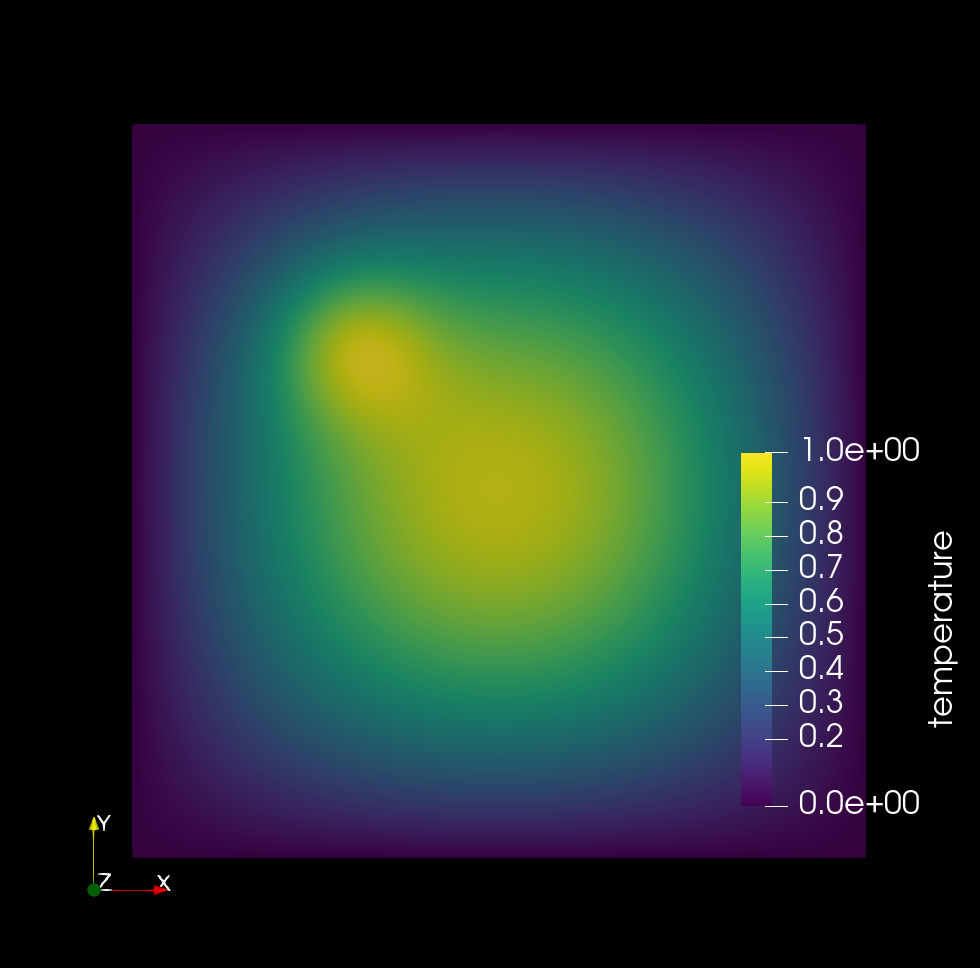
\includegraphics[width=\linewidth]{heat_t0.png}
    \caption[Heat $t\!\approx\!0$]{Heat equation at an early time: this frame exists to show that the
    implicit Euler + five-point Laplacian discretization produces a smooth, physically
    plausible temperature field on the unit square. It matters because it is the
    \emph{visual} counterpart to the iteration/residual logs: if the field were
    jagged or violated boundary conditions, the solver diagnostics would be harder to
    trust. The bright interior and darker boundary banding reflect the chosen initial
    bump and homogeneous Dirichlet boundaries---exactly the qualitative behavior
    expected before studying later-time diffusion.}
    \label{fig:heat}
  \end{subfigure}
  \hfill
  \begin{subfigure}{0.45\textwidth}
    \centering
    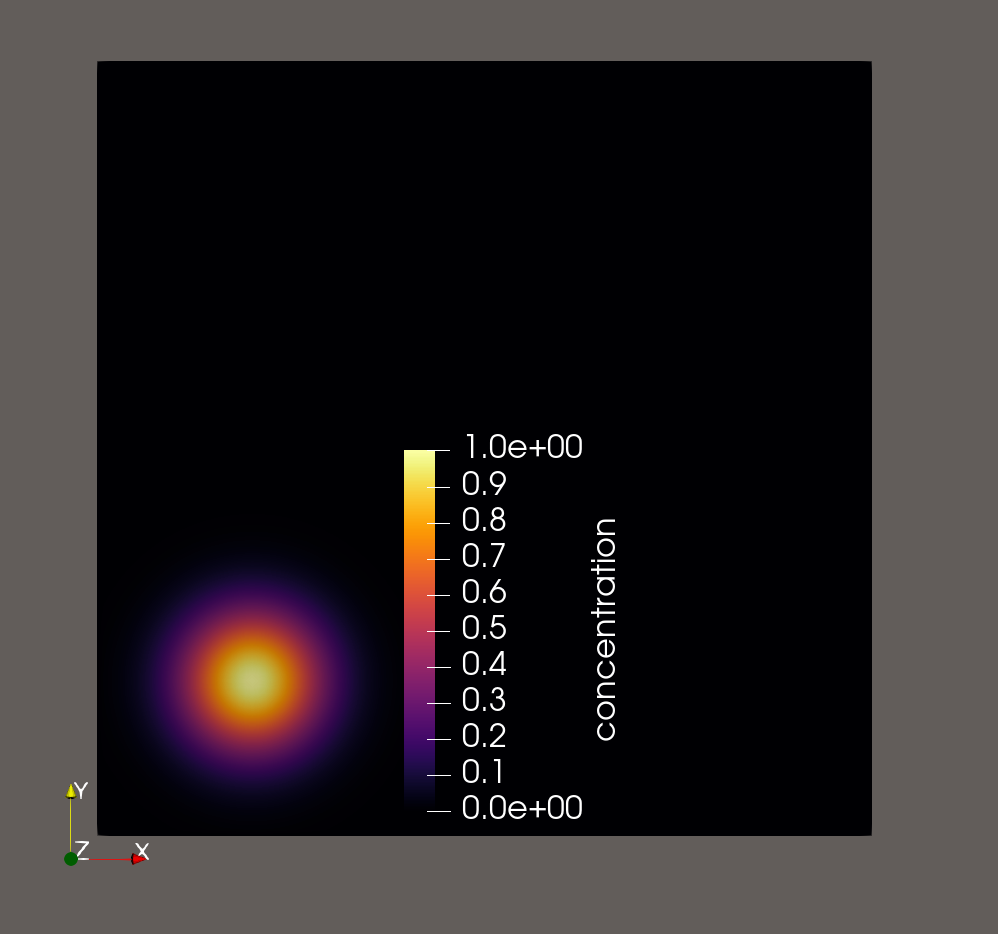
\includegraphics[width=\linewidth]{advection_diffusion_volume.png}
    \caption[Advection--diffusion snapshot]{Advection--diffusion concentration: this snapshot ties the
    nonsymmetric implicit step (upwind-like advection + diffusion) to a spatial
    pattern you can \emph{see}. It is important because it makes the course's warning
    about parallel ILU vs.\ Jacobi tangible: the field is the outcome of the same
    Krylov solve whose iteration counts we later sweep. The ``hills'' and drifted
    structure read as combined transport and spreading---if the velocity field were
    turned off, the plume would relax toward a simpler diffusion patch.}
    \label{fig:advdiff}
  \end{subfigure}

  \caption[PDE snapshots]{Representative PETSc-driven PDE snapshots exported to VTK
  surface polylines (\texttt{.vtp}) and opened in ParaView. Together they support
  the narrative that PETSc workloads are not only \texttt{KSP} counters: they are
  fields whose shape can be checked by eye against boundary conditions and qualitative
  stability.}
  \label{fig:snapshots}
\end{figure}

\begin{figure}[!h]
  \centering
  \begin{subfigure}{0.48\textwidth}
    \centering
    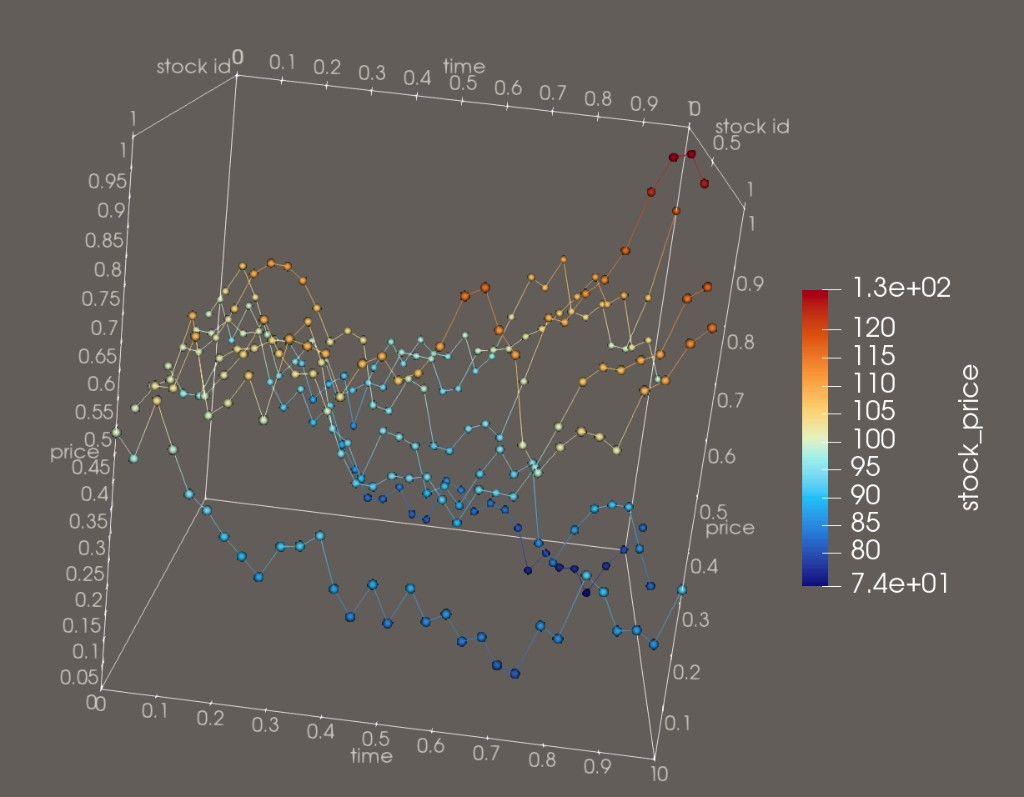
\includegraphics[width=\linewidth]{paraview_path_bundle_vtp.png}
    \caption[Path bundle, price coloring]{GBM \texttt{path\_bundle.vtp} (Monte Carlo exporter): lines are
    individual simulated paths embedded in a normalized $(t,S,z)$ frame so the
    camera is not dominated by a single long axis. Coloring by \texttt{stock\_price}
    highlights where paths explore in price space over time. This matters because it
    is the bridge claim of the report in miniature---\textbf{many independent samples}
    of the same Markovian dynamics---and the rainbow ``feathers'' read as ensemble
    dispersion: wider color spread at later times corresponds to lognormal variance
    growth.}
    \label{fig:paraview-path-price}
  \end{subfigure}
  \hfill
  \begin{subfigure}{0.48\textwidth}
    \centering
    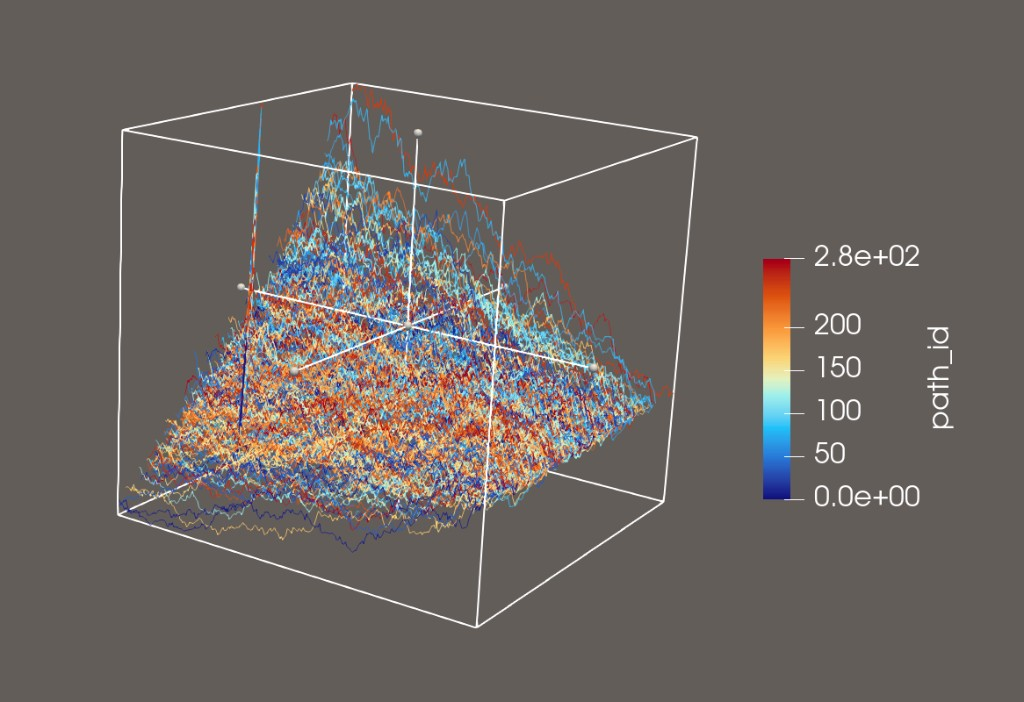
\includegraphics[width=\linewidth]{paraview_path_bundle_path_id.png}
    \caption[Path bundle, path ID]{Same geometry with \texttt{path\_id} as the scalar: each path is a
    constant hue along its polyline, which makes the \textbf{parallel batch structure}
    obvious (paths are indexed lanes). It supports the MPI narrative later---before
    ranks exist in PETSc, we already partition work by path index. The dense bundle
    shape should look like a correlated forest, not a surface: if it looked like a
    triangulated sheet, that would indicate a wrong ParaView representation (e.g.\
    triangulating points as a surface).}
    \label{fig:paraview-path-pid}
  \end{subfigure}
  \caption[Monte Carlo path bundle in ParaView]{Monte Carlo path bundle (\texttt{path\_bundle.vtp}): two
  equivalent views of the same polylines, emphasizing either physical economics
  (\texttt{stock\_price}) or implementation partitioning (\texttt{path\_id}).}
  \label{fig:paraview-mc-bundle}
\end{figure}

\begin{figure}[!h]
  \centering
  \begin{subfigure}{0.32\textwidth}
    \centering
    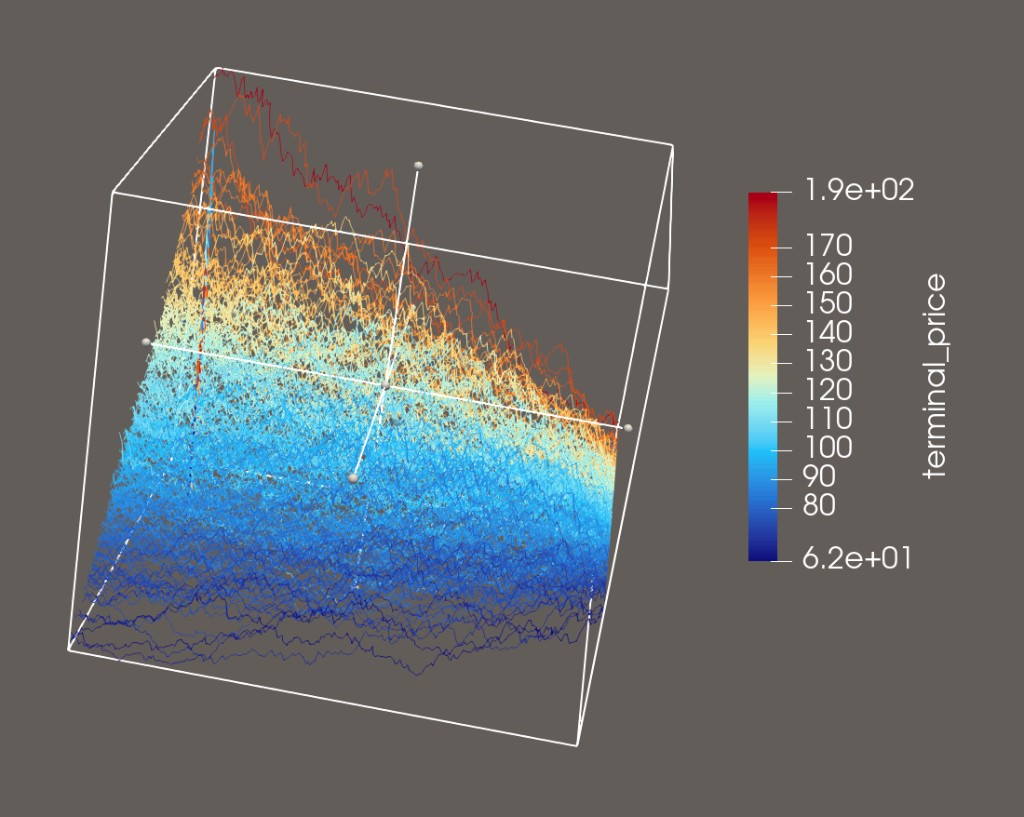
\includegraphics[width=\linewidth]{paraview_path_bundle_terminal_price.png}
    \caption{\texttt{terminal\_price} (per-path terminal level, replicated along the
    polyline) encodes where each path ends in spot space; warm colors are higher
    terminal draws. It links the time-sliced view to the \textbf{payoff input} that
    actually drives European-style summaries.}
    \label{fig:pv-term}
  \end{subfigure}
  \hfill
  \begin{subfigure}{0.32\textwidth}
    \centering
    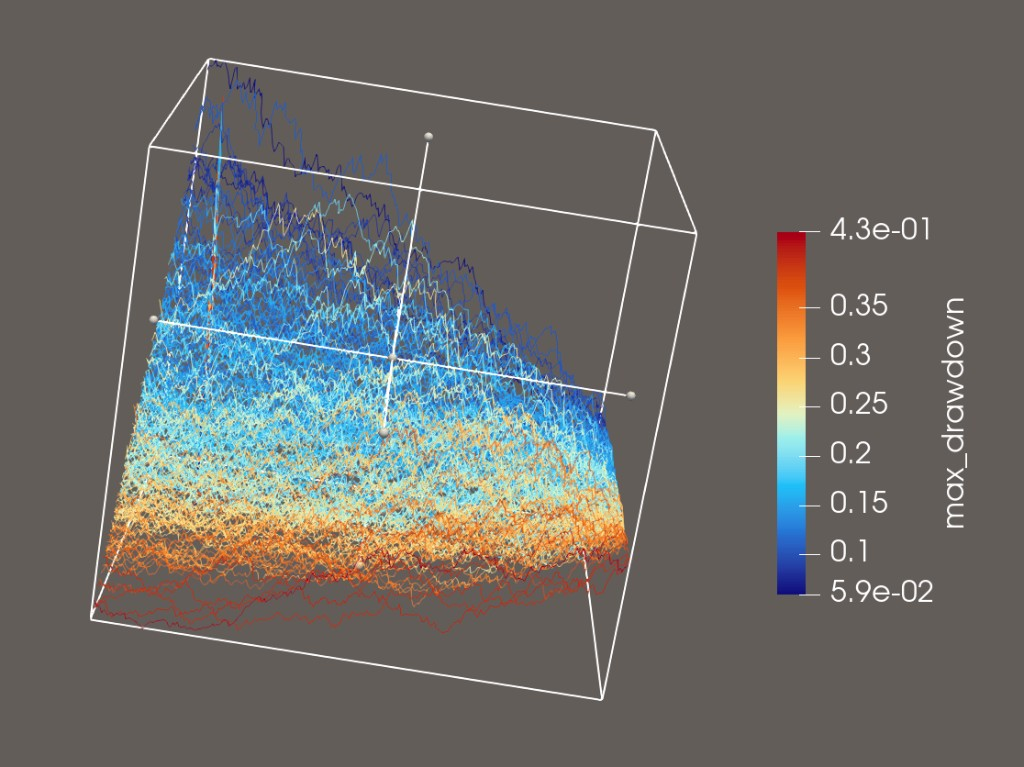
\includegraphics[width=\linewidth]{paraview_max_drawdown.png}
    \caption{\texttt{max\_drawdown} summarizes pathwise depth of drawdowns; larger
    values (warmer) are paths that dipped far below their running maximum before
    recovering. It matters for risk narratives beyond the terminal value alone.}
    \label{fig:pv-dd}
  \end{subfigure}
  \hfill
  \begin{subfigure}{0.32\textwidth}
    \centering
    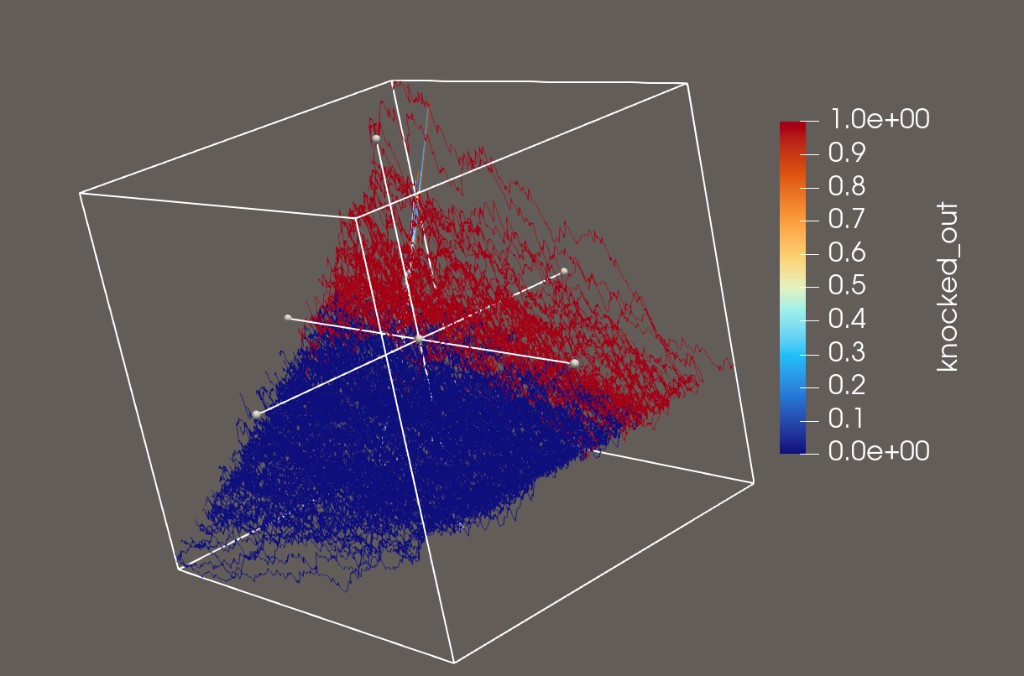
\includegraphics[width=\linewidth]{paraview_knocked_out.png}
    \caption{\texttt{knocked\_out} is essentially binary here: paths that touched the
    barrier level are one color, survivors another. The split should read as
    \textbf{geometry interacting with a threshold}, analogous to barrier option
    knock-out events.}
    \label{fig:pv-ko}
  \end{subfigure}
  \caption[Stock-path bundle scalars]{Enriched GBM export (\texttt{stock\_paths.vtp}): pathwise summaries
  exposed as point fields so ParaView can color tubes/lines without CSV gymnastics.
  These panels answer ``what does the model \emph{do} to paths?'' beyond mean/variance
  reduction alone.}
  \label{fig:paraview-stock-risk}
\end{figure}

\begin{figure}[!h]
  \centering
  \begin{subfigure}{0.48\textwidth}
    \centering
    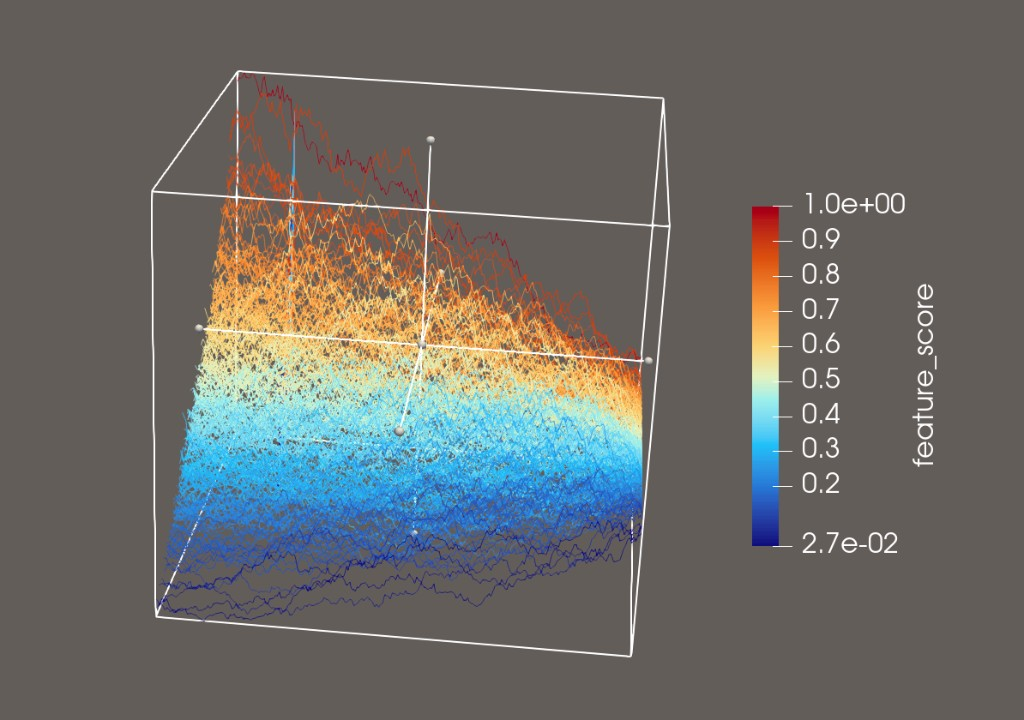
\includegraphics[width=\linewidth]{paraview_feature_score.png}
    \caption{\texttt{feature\_score} is a deliberately engineered scalar combining
    normalized terminal level, drawdown, and barrier gap (see repository exporter).
    Smooth gradients mean the chosen normalization is spreading paths across $[0,1]$;
    a degenerate flat image would mean all paths look the same under those features.}
    \label{fig:pv-fs}
  \end{subfigure}
  \hfill
  \begin{subfigure}{0.48\textwidth}
    \centering
    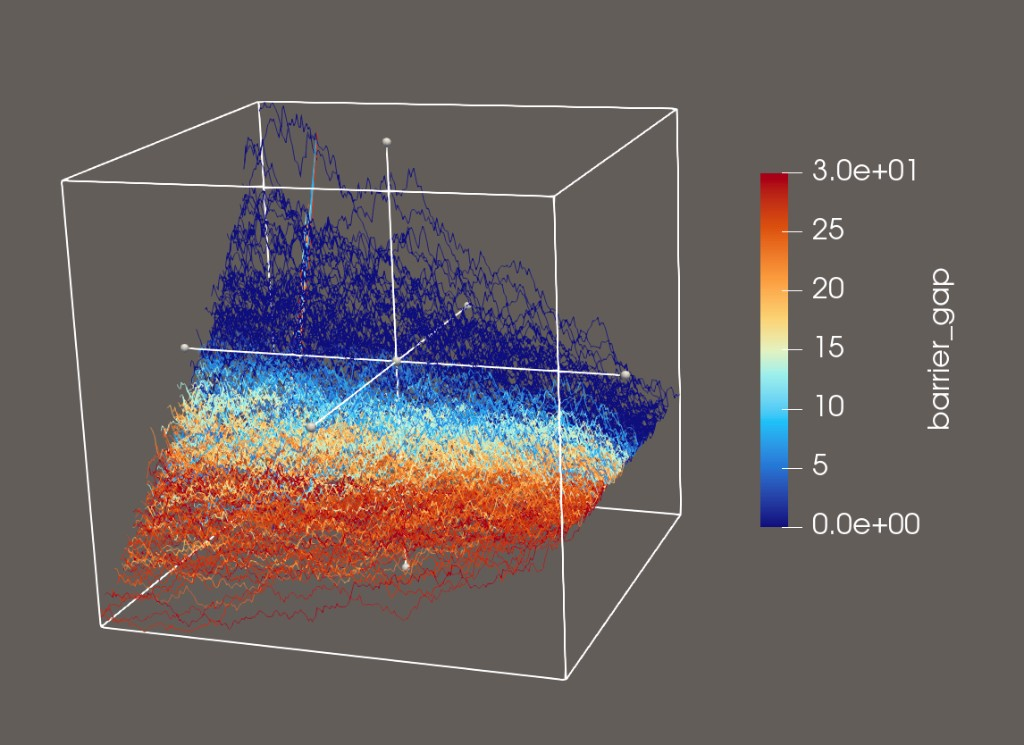
\includegraphics[width=\linewidth]{paraview_barrier_gap.png}
    \caption{\texttt{barrier\_gap} measures how far a path's running maximum stayed
    \emph{below} the barrier (in price units, floored at zero). Large gaps (warm)
    mean ``never came close''; small gaps mean near-touching---the visual complement
    to knock-out indicators.}
    \label{fig:pv-bg}
  \end{subfigure}
  \caption[Composite path-risk scalars]{Composite scalars on \texttt{stock\_paths.vtp}: these are not
  standard textbook fields; they are \textbf{reporting aids} that compress several
  path statistics into a single colormap for storytelling.}
  \label{fig:paraview-stock-geom}
\end{figure}

\begin{figure}[!h]
  \centering
  \begin{subfigure}{0.48\textwidth}
    \centering
    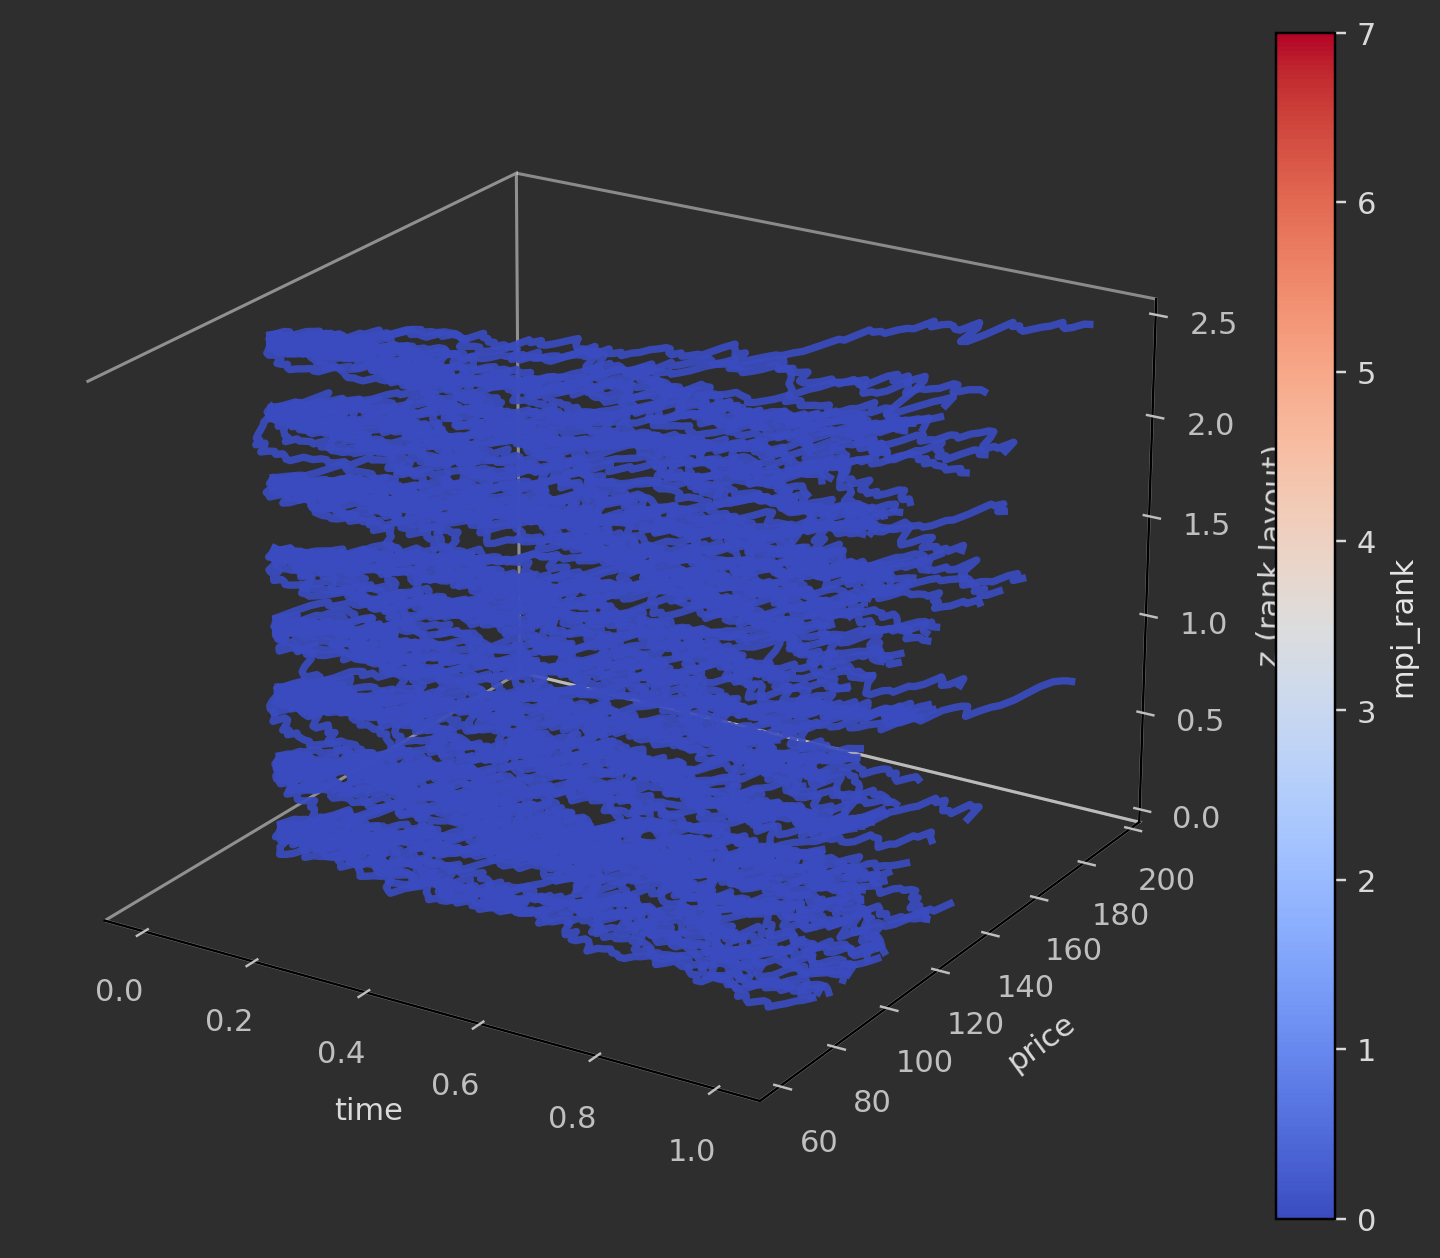
\includegraphics[width=\linewidth]{paraview_mpi_domain_paths.png}
    \caption[Synthetic MPI batches]{Synthetic ``MPI rank'' coloring of path batches (\texttt{mpi\_domain\_paths.vtp}).
    \textbf{Context:} the exporter tags each path batch with an integer rank for
    visualization only. \textbf{Why it matters:} it makes the SPMD \emph{decomposition}
    metaphor visible before jumping to mesh partitioning. \textbf{How to read it:}
    separated hue families mean batches are distinct; this is not literal
    \texttt{MPI\_COMM\_WORLD} telemetry from a solver run.}
    \label{fig:pv-mpi-default}
  \end{subfigure}
  \hfill
  \begin{subfigure}{0.48\textwidth}
    \centering
    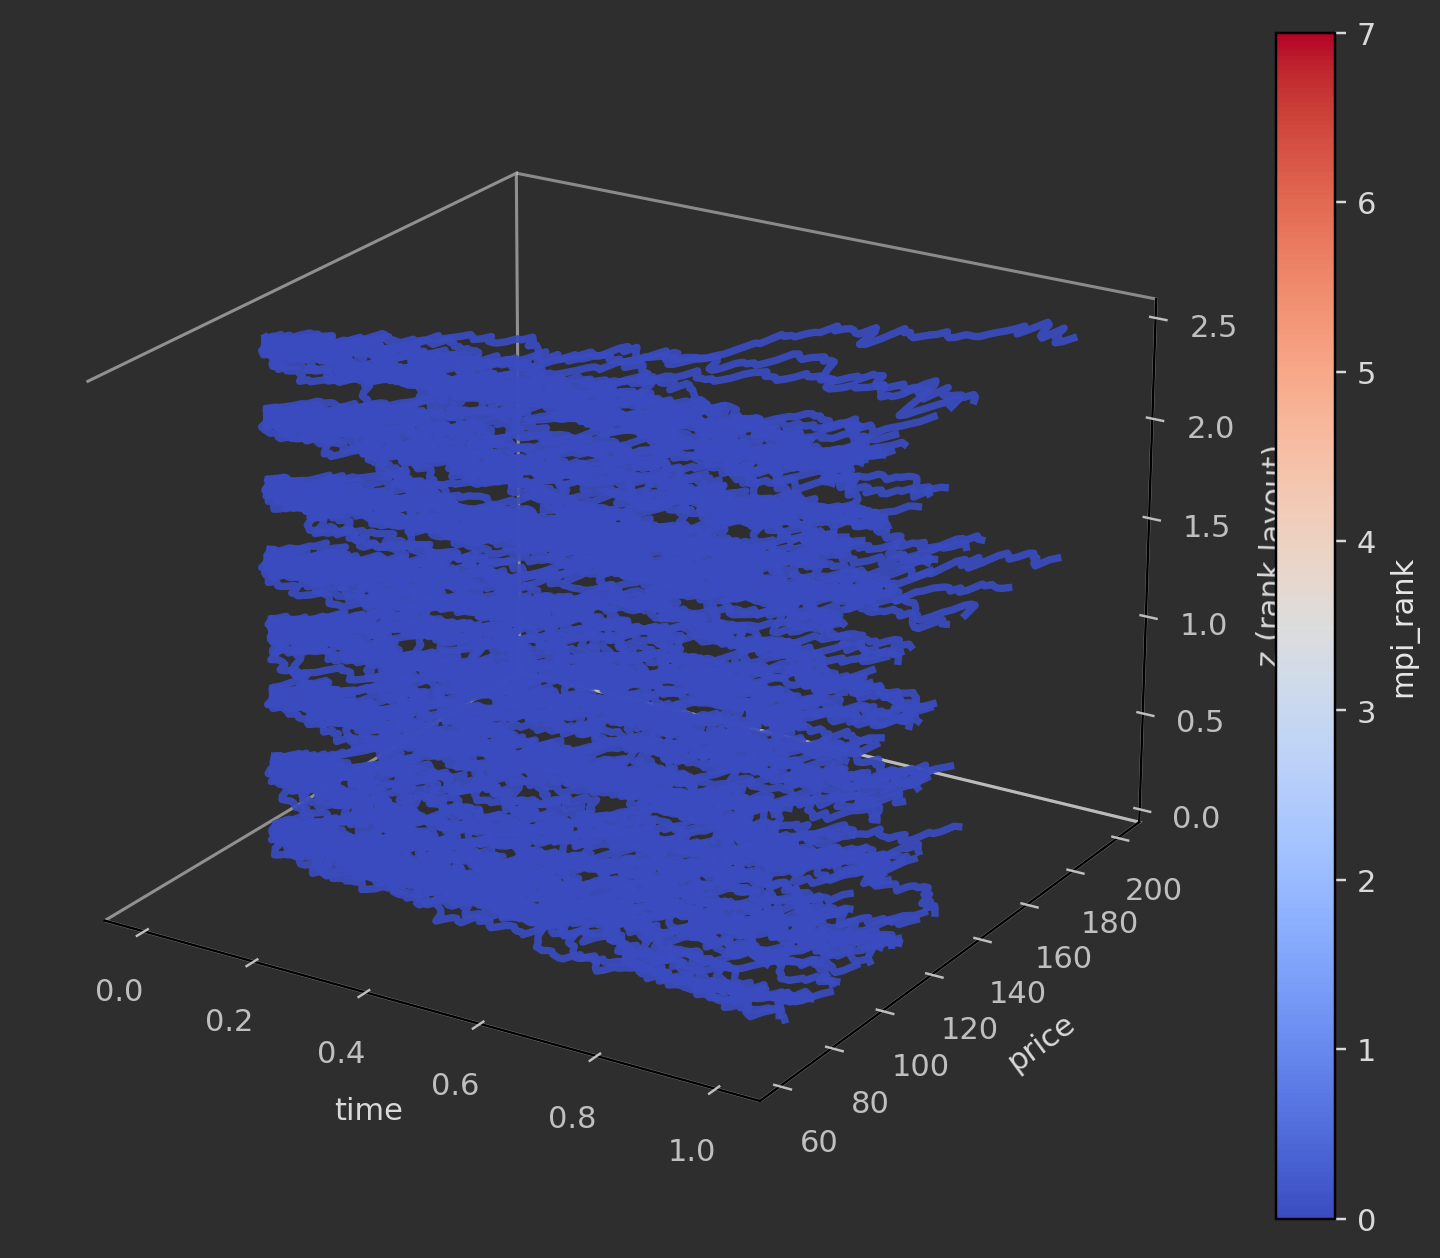
\includegraphics[width=\linewidth]{paraview_mpi_pretty.png}
    \caption[Pretty MPI paths]{``Pretty'' parameters (more paths/steps) for the same synthetic rank
    coloring (\texttt{pretty\_mpi\_domain\_paths.vtp}). Denser bundles emphasize how
    rank-separated batches fill space when the workload increases---useful for
    presentations even though the underlying model remains stylized GBM.}
    \label{fig:pv-mpi-pretty}
  \end{subfigure}
  \caption[Synthetic MPI path metaphor]{MPI path metaphor (matplotlib render of polylines with cool--warm
  coloring by \texttt{mpi\_rank}; see \texttt{scripts/render\_mpi\_paths\_png.py}).
  These figures exist so the PDF carries a visual even when native ParaView Tube
  screenshots are not embedded.}
  \label{fig:paraview-mpi}
\end{figure}

\newpage
\section{Figures: Monte Carlo and HPC dashboards}
\label{sec:figures-mc}

\begin{figure}[!h]
  \centering
  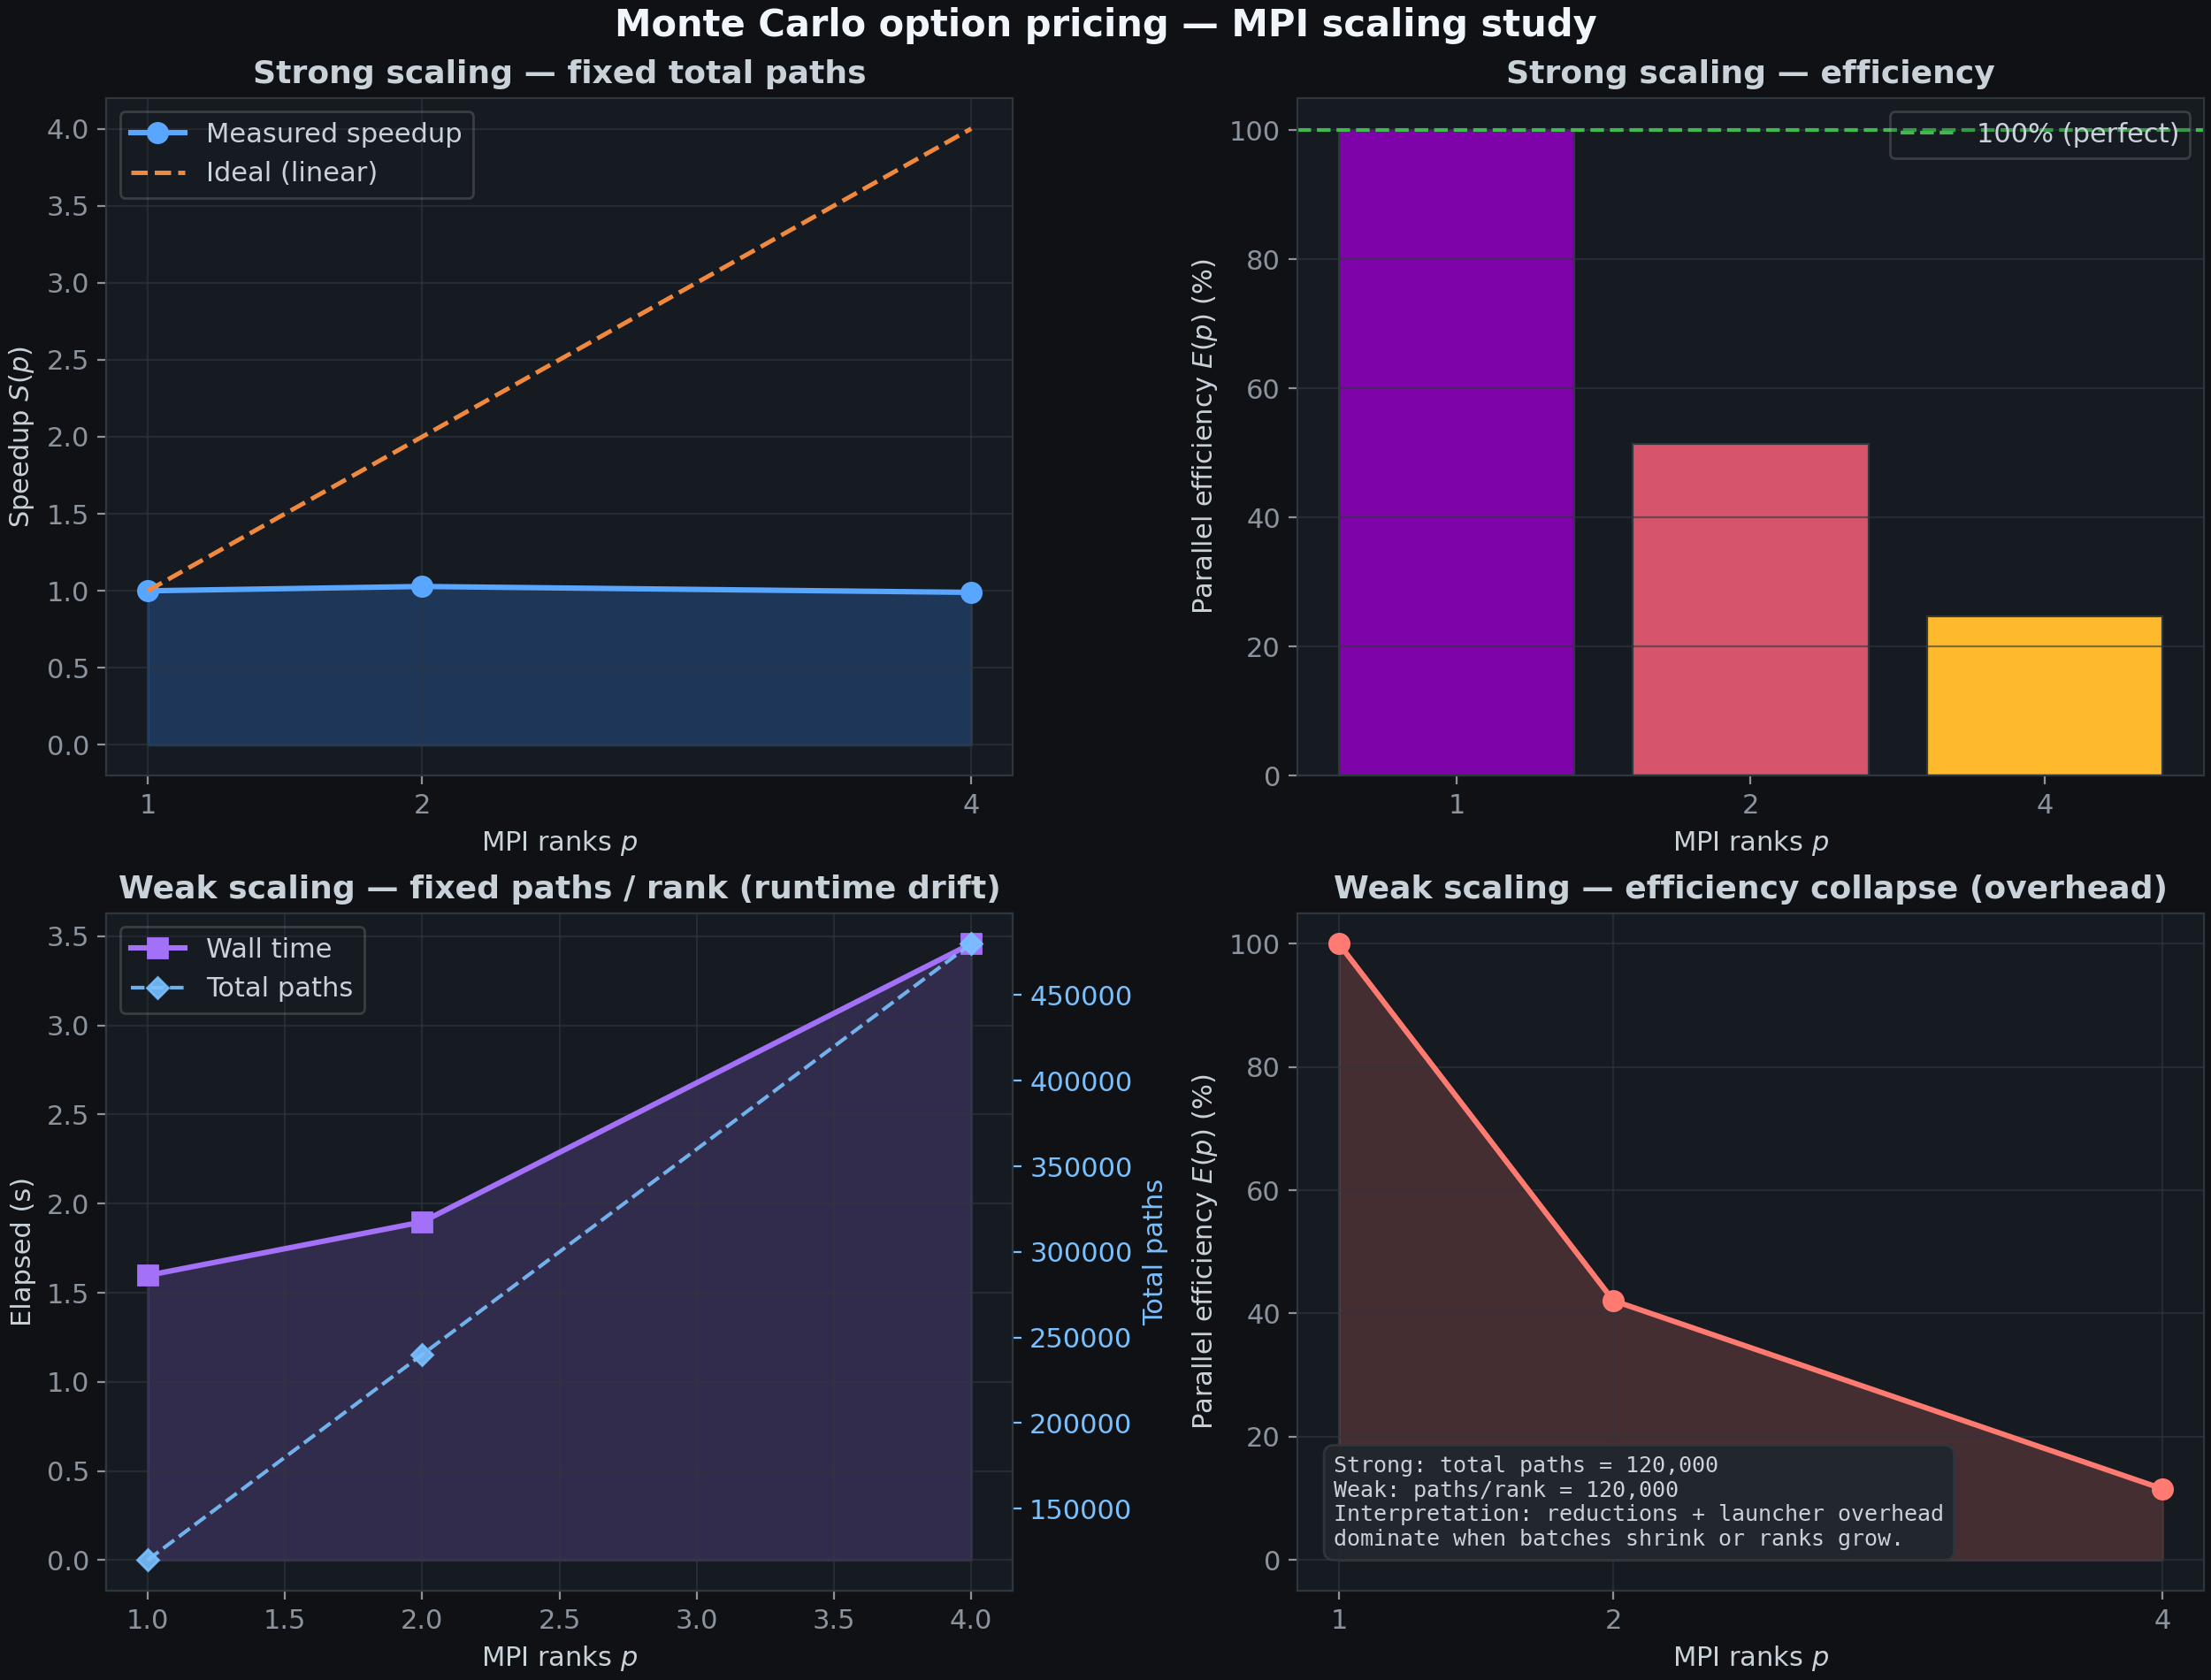
\includegraphics[width=\figw]{hpc_scaling_dashboard.png}
  \caption[HPC scaling dashboard]{HPC scaling dashboard: this figure compresses strong and weak scaling
  experiments into one glanceable page. \textbf{Context:} it summarizes timings and
  speedups from the repository's scaling drivers. \textbf{Why it matters:} parallel
  MC is not automatically linear speedup---collectives, load balance, and fixed problem
  size all bend the curves. \textbf{How to read it:} near-linear segments mean
  additional ranks buy wall time; flattening or downturns mean communication or
  insufficient work per rank dominates.}
  \label{fig:hpc-dashboard}
\end{figure}

\begin{figure}[!h]
  \centering
  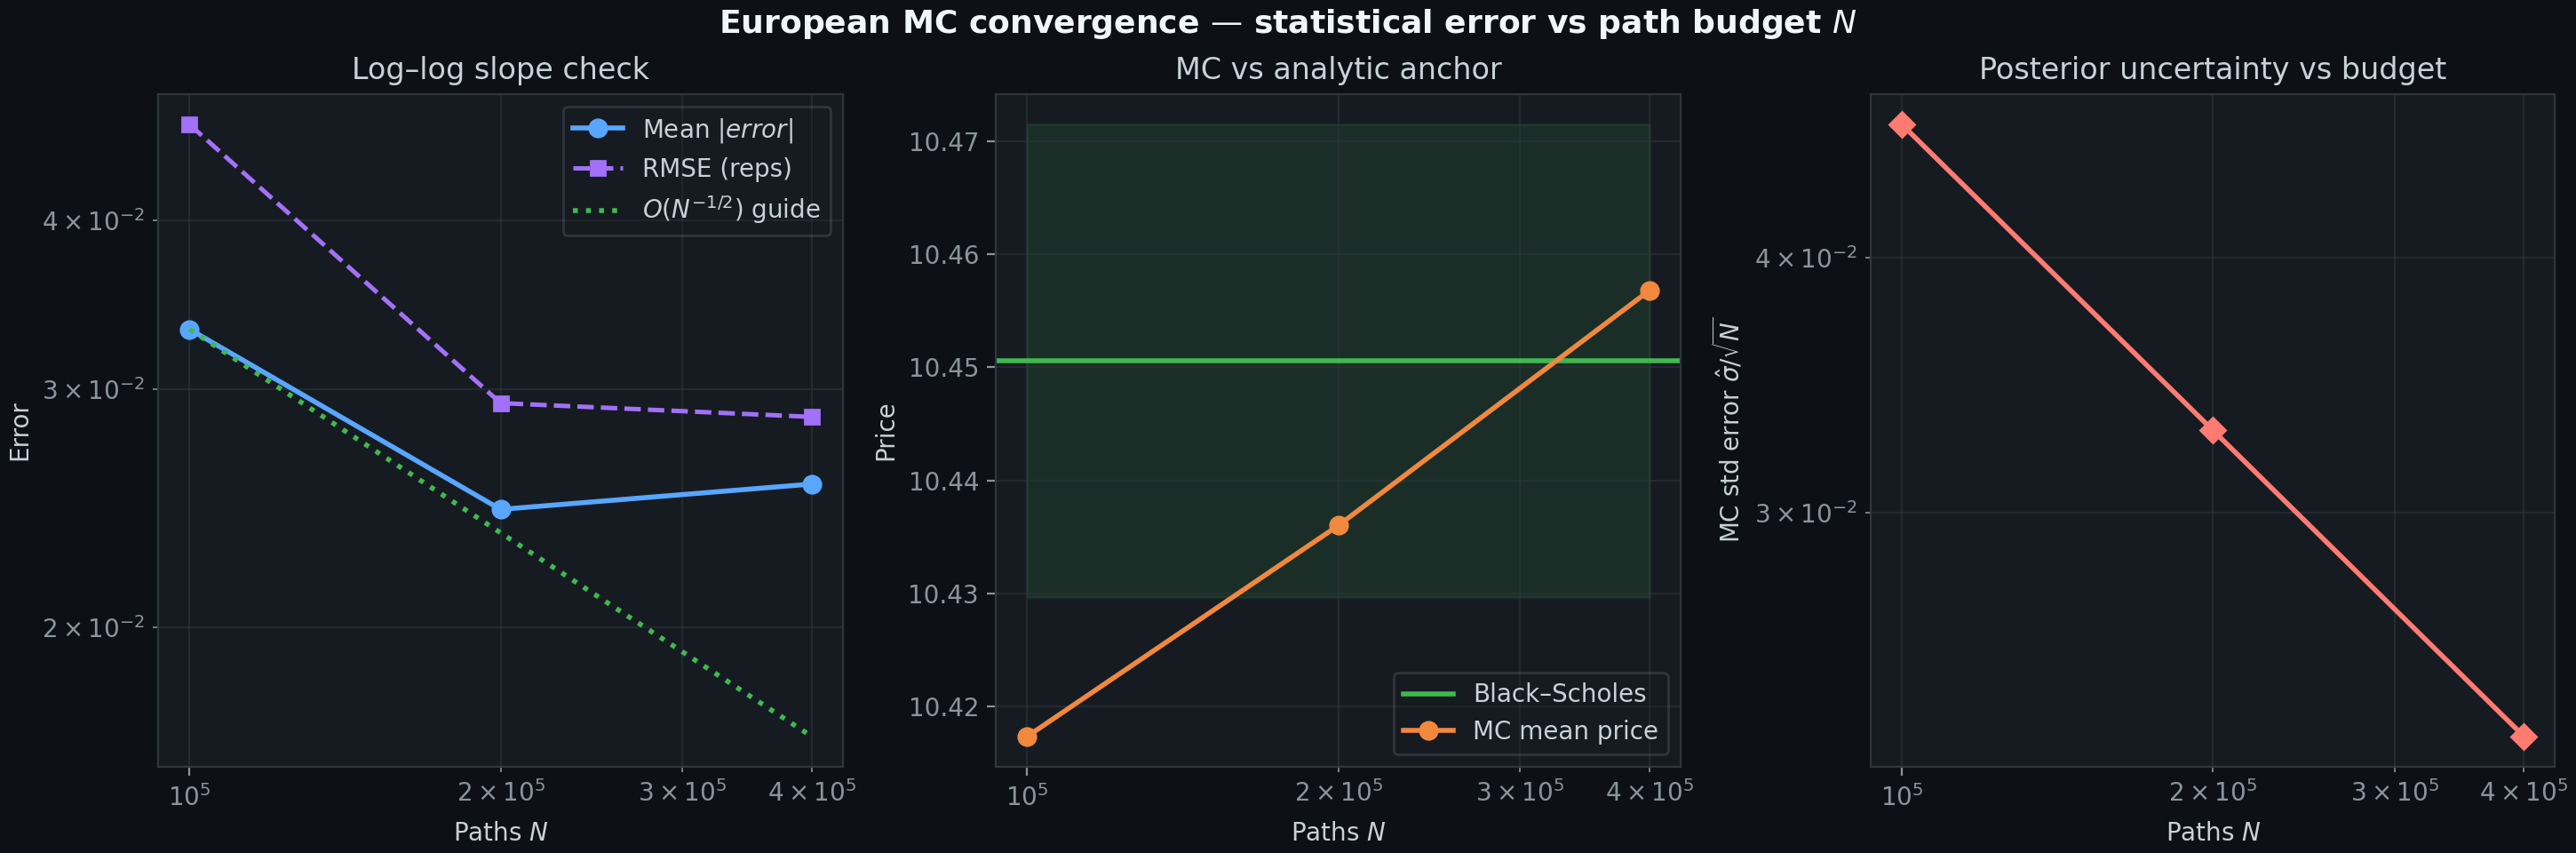
\includegraphics[width=\figw]{hpc_convergence_triptych.png}
  \caption[MC convergence triptych]{Monte Carlo convergence triptych vs.\ Black--Scholes: each panel fixes a
  viewpoint (price error, stderr, relative error) while varying $N$ or method
  knobs. It is the statistical counterpart to the PDE mesh-refinement story---we
  expect $O(N^{-1/2})$ decay of Monte Carlo error, not machine precision. Curves that
  flatten early usually mean the trial stopped before the asymptotic regime or that
  variance reduction changed the prefactor.}
  \label{fig:hpc-conv}
\end{figure}

\begin{figure}[!h]

  \centering

  \begin{subfigure}{0.4\textwidth}

    \centering

    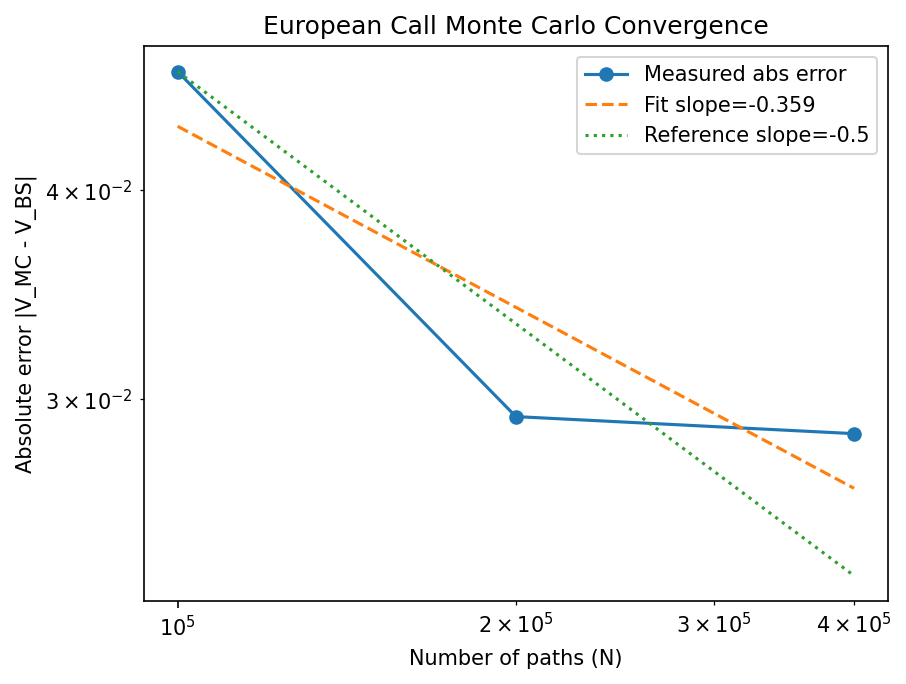
\includegraphics[width=\linewidth]{convergence.png}

    \caption[Error vs.\ $N$]{Monte Carlo error vs.\ path count $N$ on log--log scales. A line near slope
    $-1/2$ is the signature of square-root Monte Carlo error decay; systematic offsets
    between markers usually mean different RNG streams, antithetic pairing, or
    payoff implementations---not ``better physics'' by themselves.}

    \label{fig:conv-n}

  \end{subfigure}

  \hfill

  \begin{subfigure}{0.4\textwidth}

    \centering
    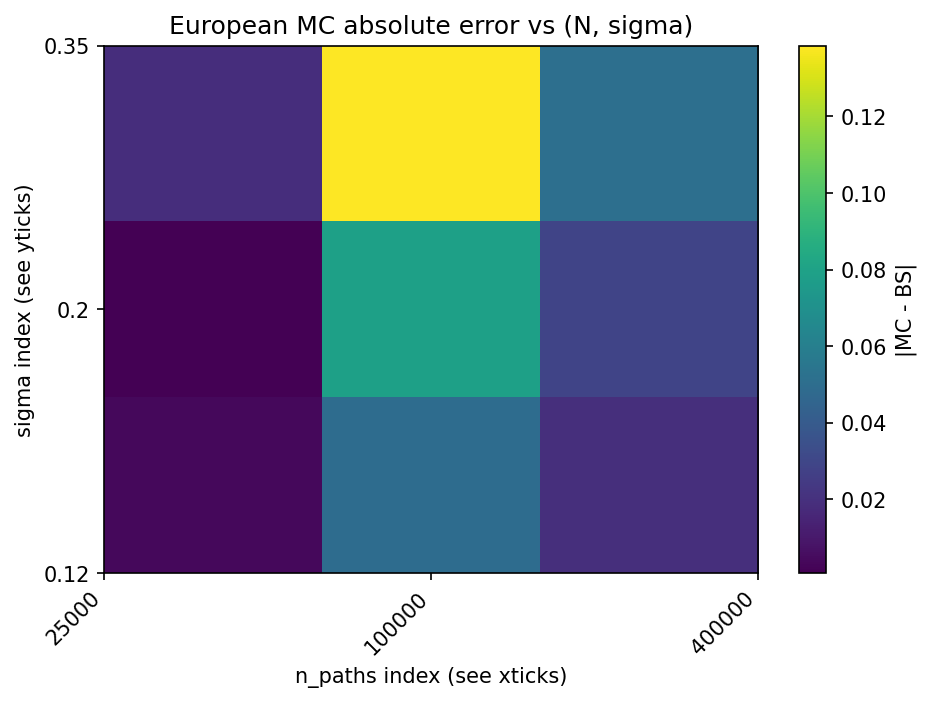
\includegraphics[width=\linewidth]{error_surface_abs_err.png}

    \caption[Error surface]{Absolute error over $(N,\sigma)$: this surface makes the \textbf{coupled}
    sensitivity to both sample count and volatility visible. Ridges or hot spots
    flag regimes where either sampling is insufficient or $\sigma$ moves the payoff
    into a harder region (e.g.\ near the money with large diffusion).}

    \label{fig:error-surface}

  \end{subfigure}

  \caption[European MC error summary]{European Monte Carlo convergence and absolute error comparison against
  Black--Scholes: together the panels connect \emph{statistical} error budgets to a
  two-parameter experimental sweep, mirroring how practitioners explore both
  discretization and sampling uncertainty.}

  \label{fig:mc-error-summary}

\end{figure}

\begin{figure}[!h]
  \centering
  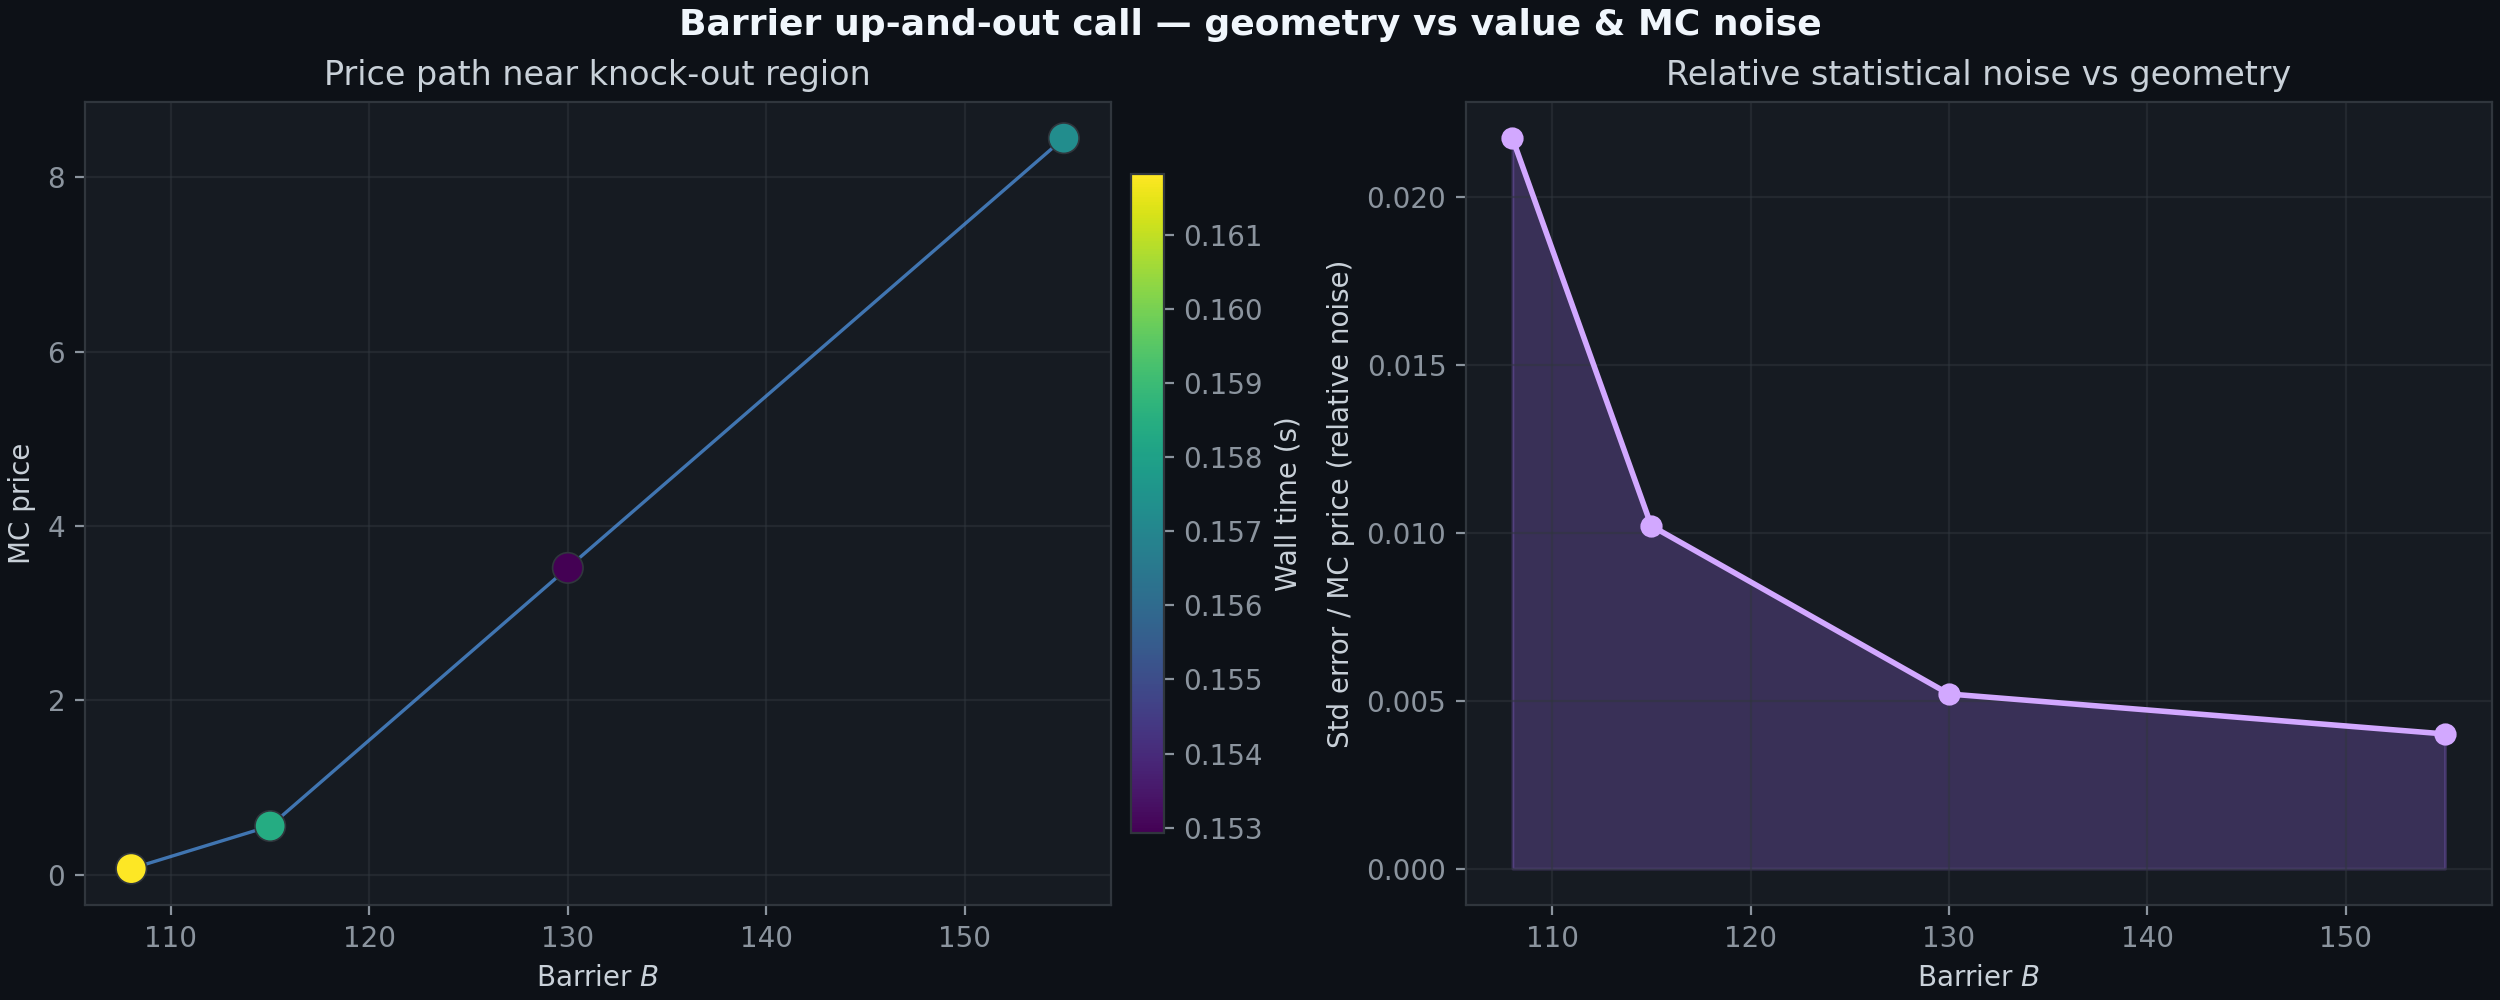
\includegraphics[width=\figw]{hpc_barrier_geometry_story.png}
  \caption[Barrier sweep storyboard]{Barrier sweep storyboard: price, stderr, and geometry vs.\ barrier
  level. This is the payoff-driven variance story in visual form---as the barrier
  moves through the bulk of the terminal distribution, estimators often become
  noisier or more sensitive. A widening stderr band without a corresponding price shift
  would suggest ``statistical stress'' rather than a change in the limit value.}
  \label{fig:barrier}
\end{figure}

\begin{figure}[!h]
  \centering
  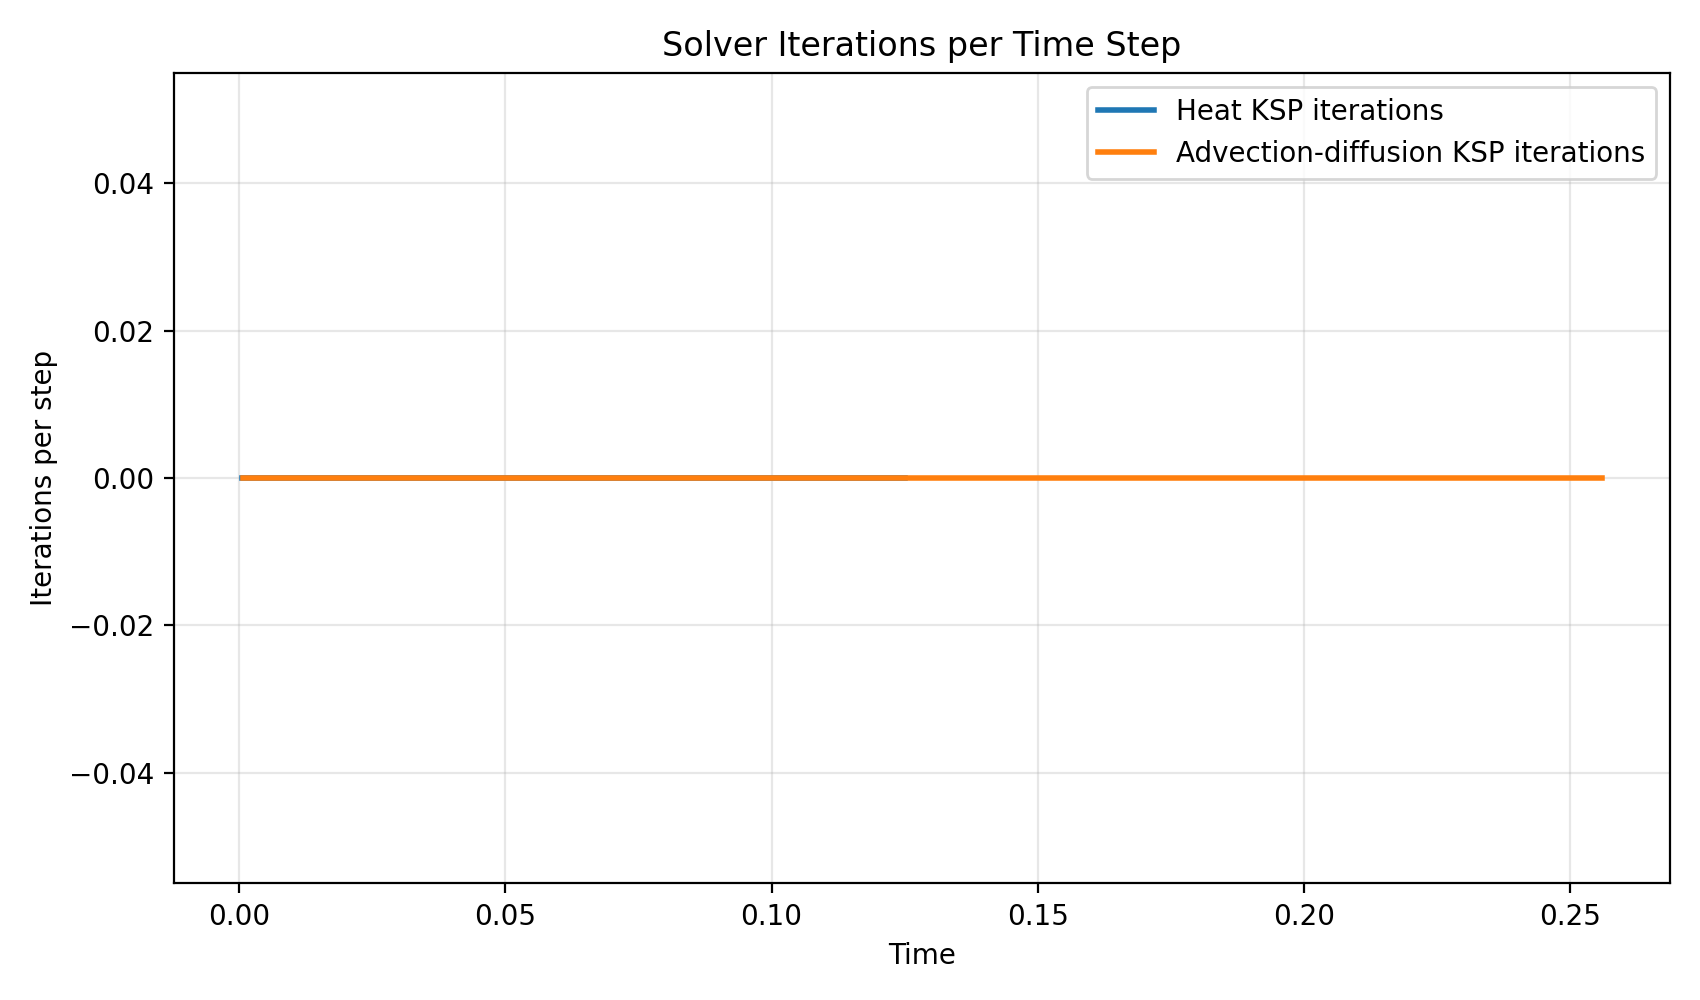
\includegraphics[width=\figw]{solver_compare_runtime.png}
  \caption[Solver vs.\ MC runtime]{Solver vs.\ Monte Carlo runtime comparison: this plot places two
  different PETSc ``worlds'' on the same axis---sampling-dominated vs.\
  linear-solve-dominated work. It matters because the report's thesis is that the
  \textbf{same engineering discipline} (honest timings, reproducible scripts) applies
  to both even when the bottleneck moves. Relative ordering that flips with problem
  size is normal: tiny linear solves are launcher-bound, while large MC runs become
  communication-bound.}
  \label{fig:solver-vs-mc}
\end{figure}

\section{Figures: Phase~2 inputs and roll-forward}

\begin{figure}[!h]
  \centering
  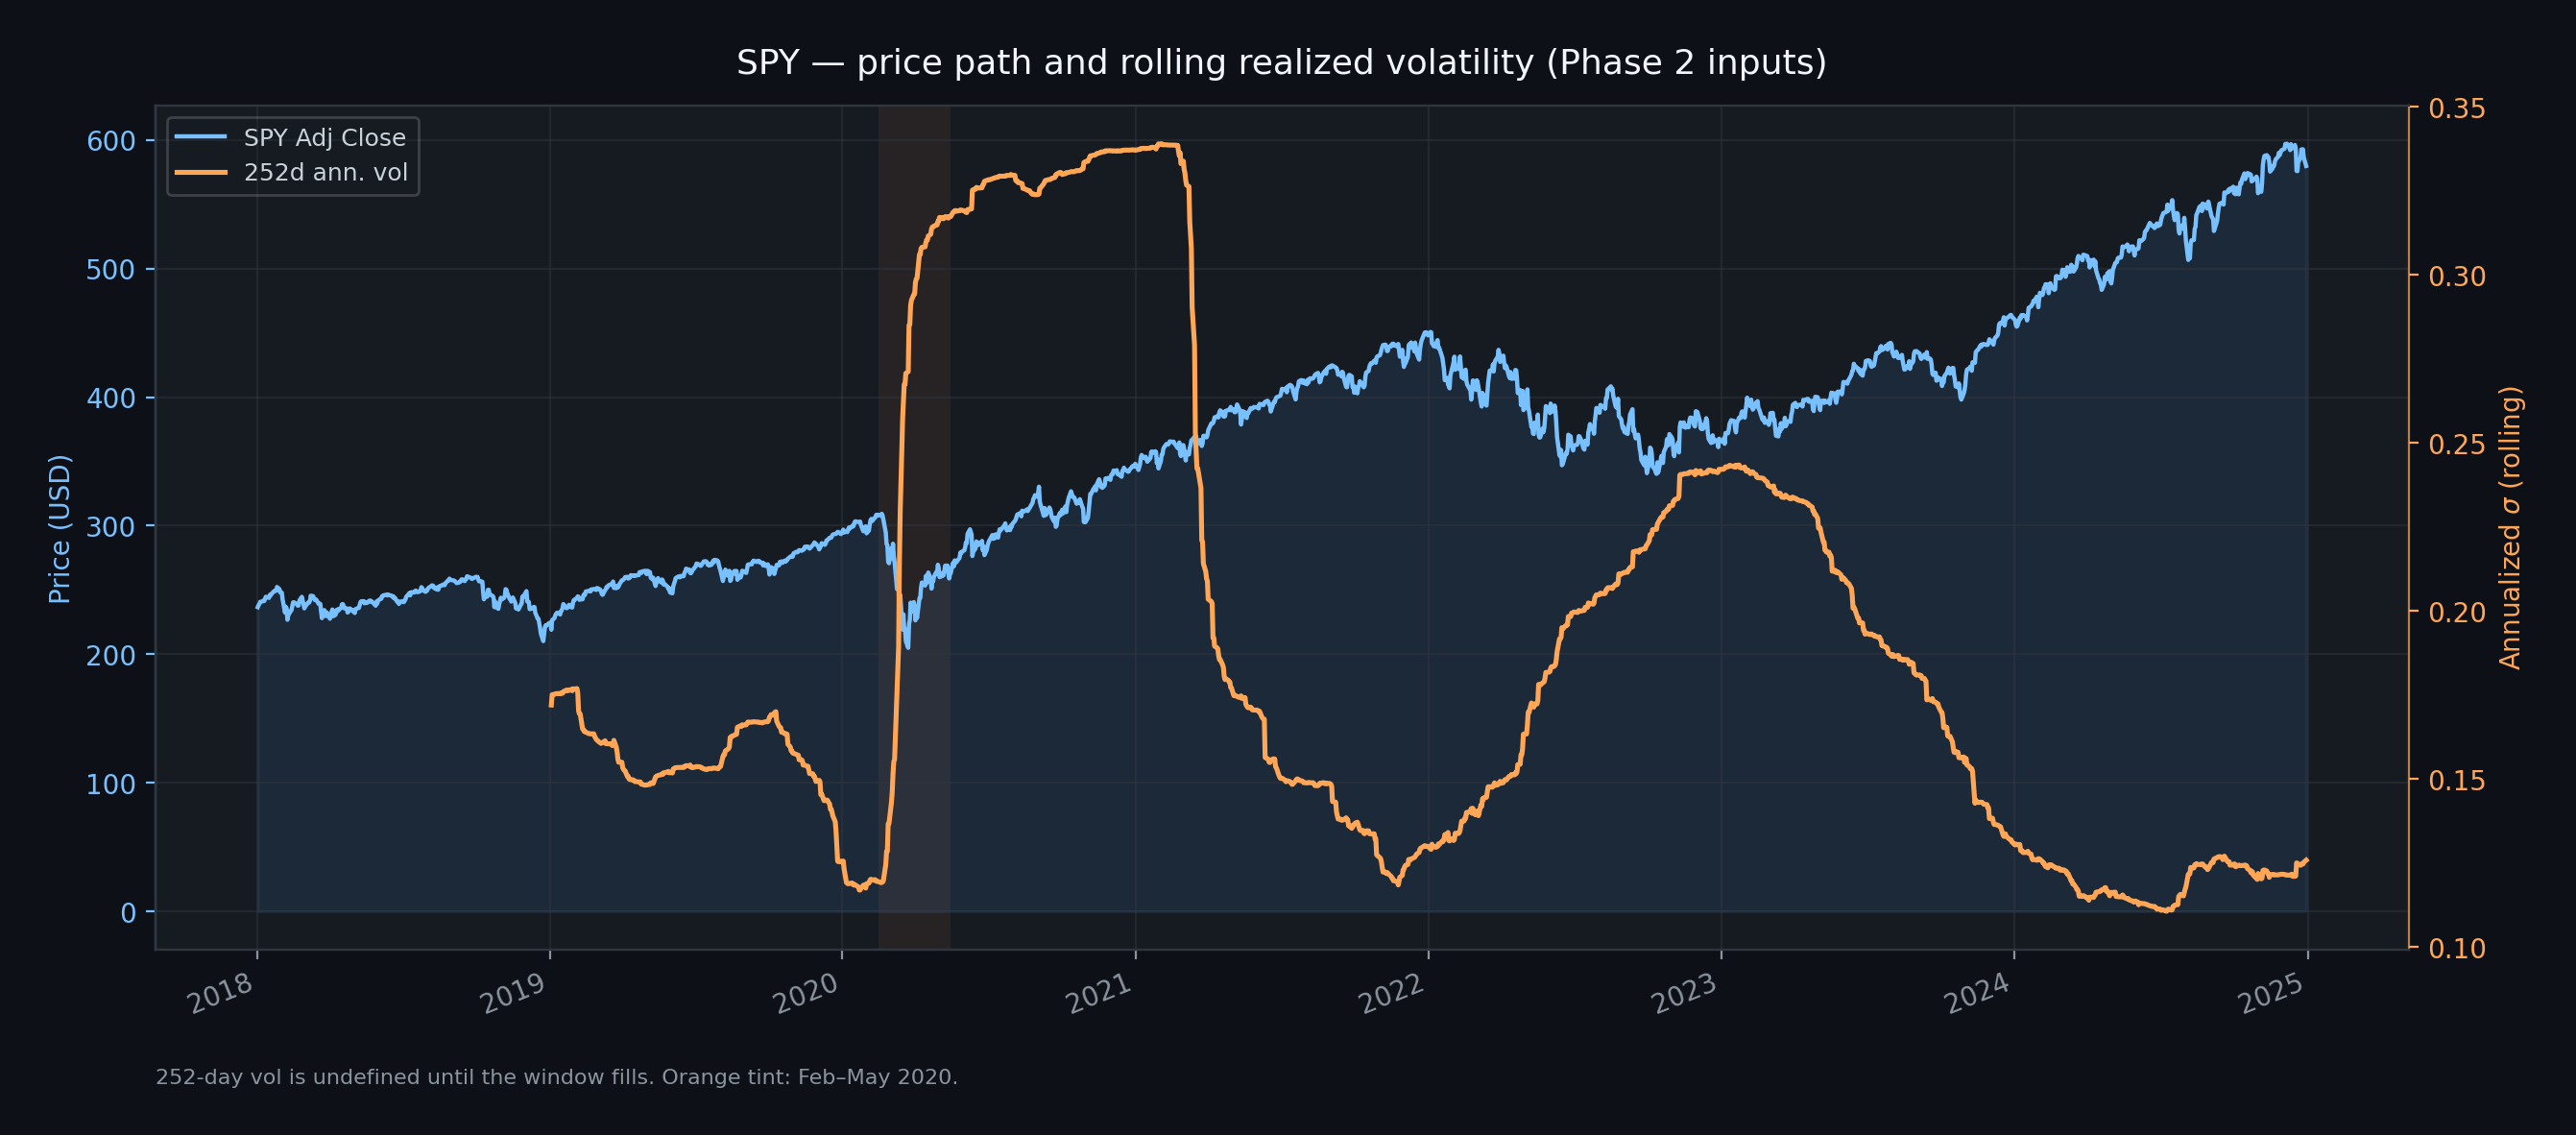
\includegraphics[width=\figw]{phase2_spy_price_and_vol.png}
  \caption[SPY and realized vol]{SPY price path with rolling $252$-day annualized realized volatility.
  \textbf{Context:} Phase~2 replaces constant $\sigma$ with a data-driven process.
  \textbf{Why it matters:} it shows \textbf{nonstationarity}---the same MC engine will
  ingest different vol inputs on different roll dates. \textbf{How to read it:}
  volatility spikes (right axis) should align visually with fast market moves
  (left axis); a flat vol line would mean the rolling window lost responsiveness or
  the data feed is incomplete.}
  \label{fig:phase2-spy}
\end{figure}

\begin{figure}[!h]
  \centering
  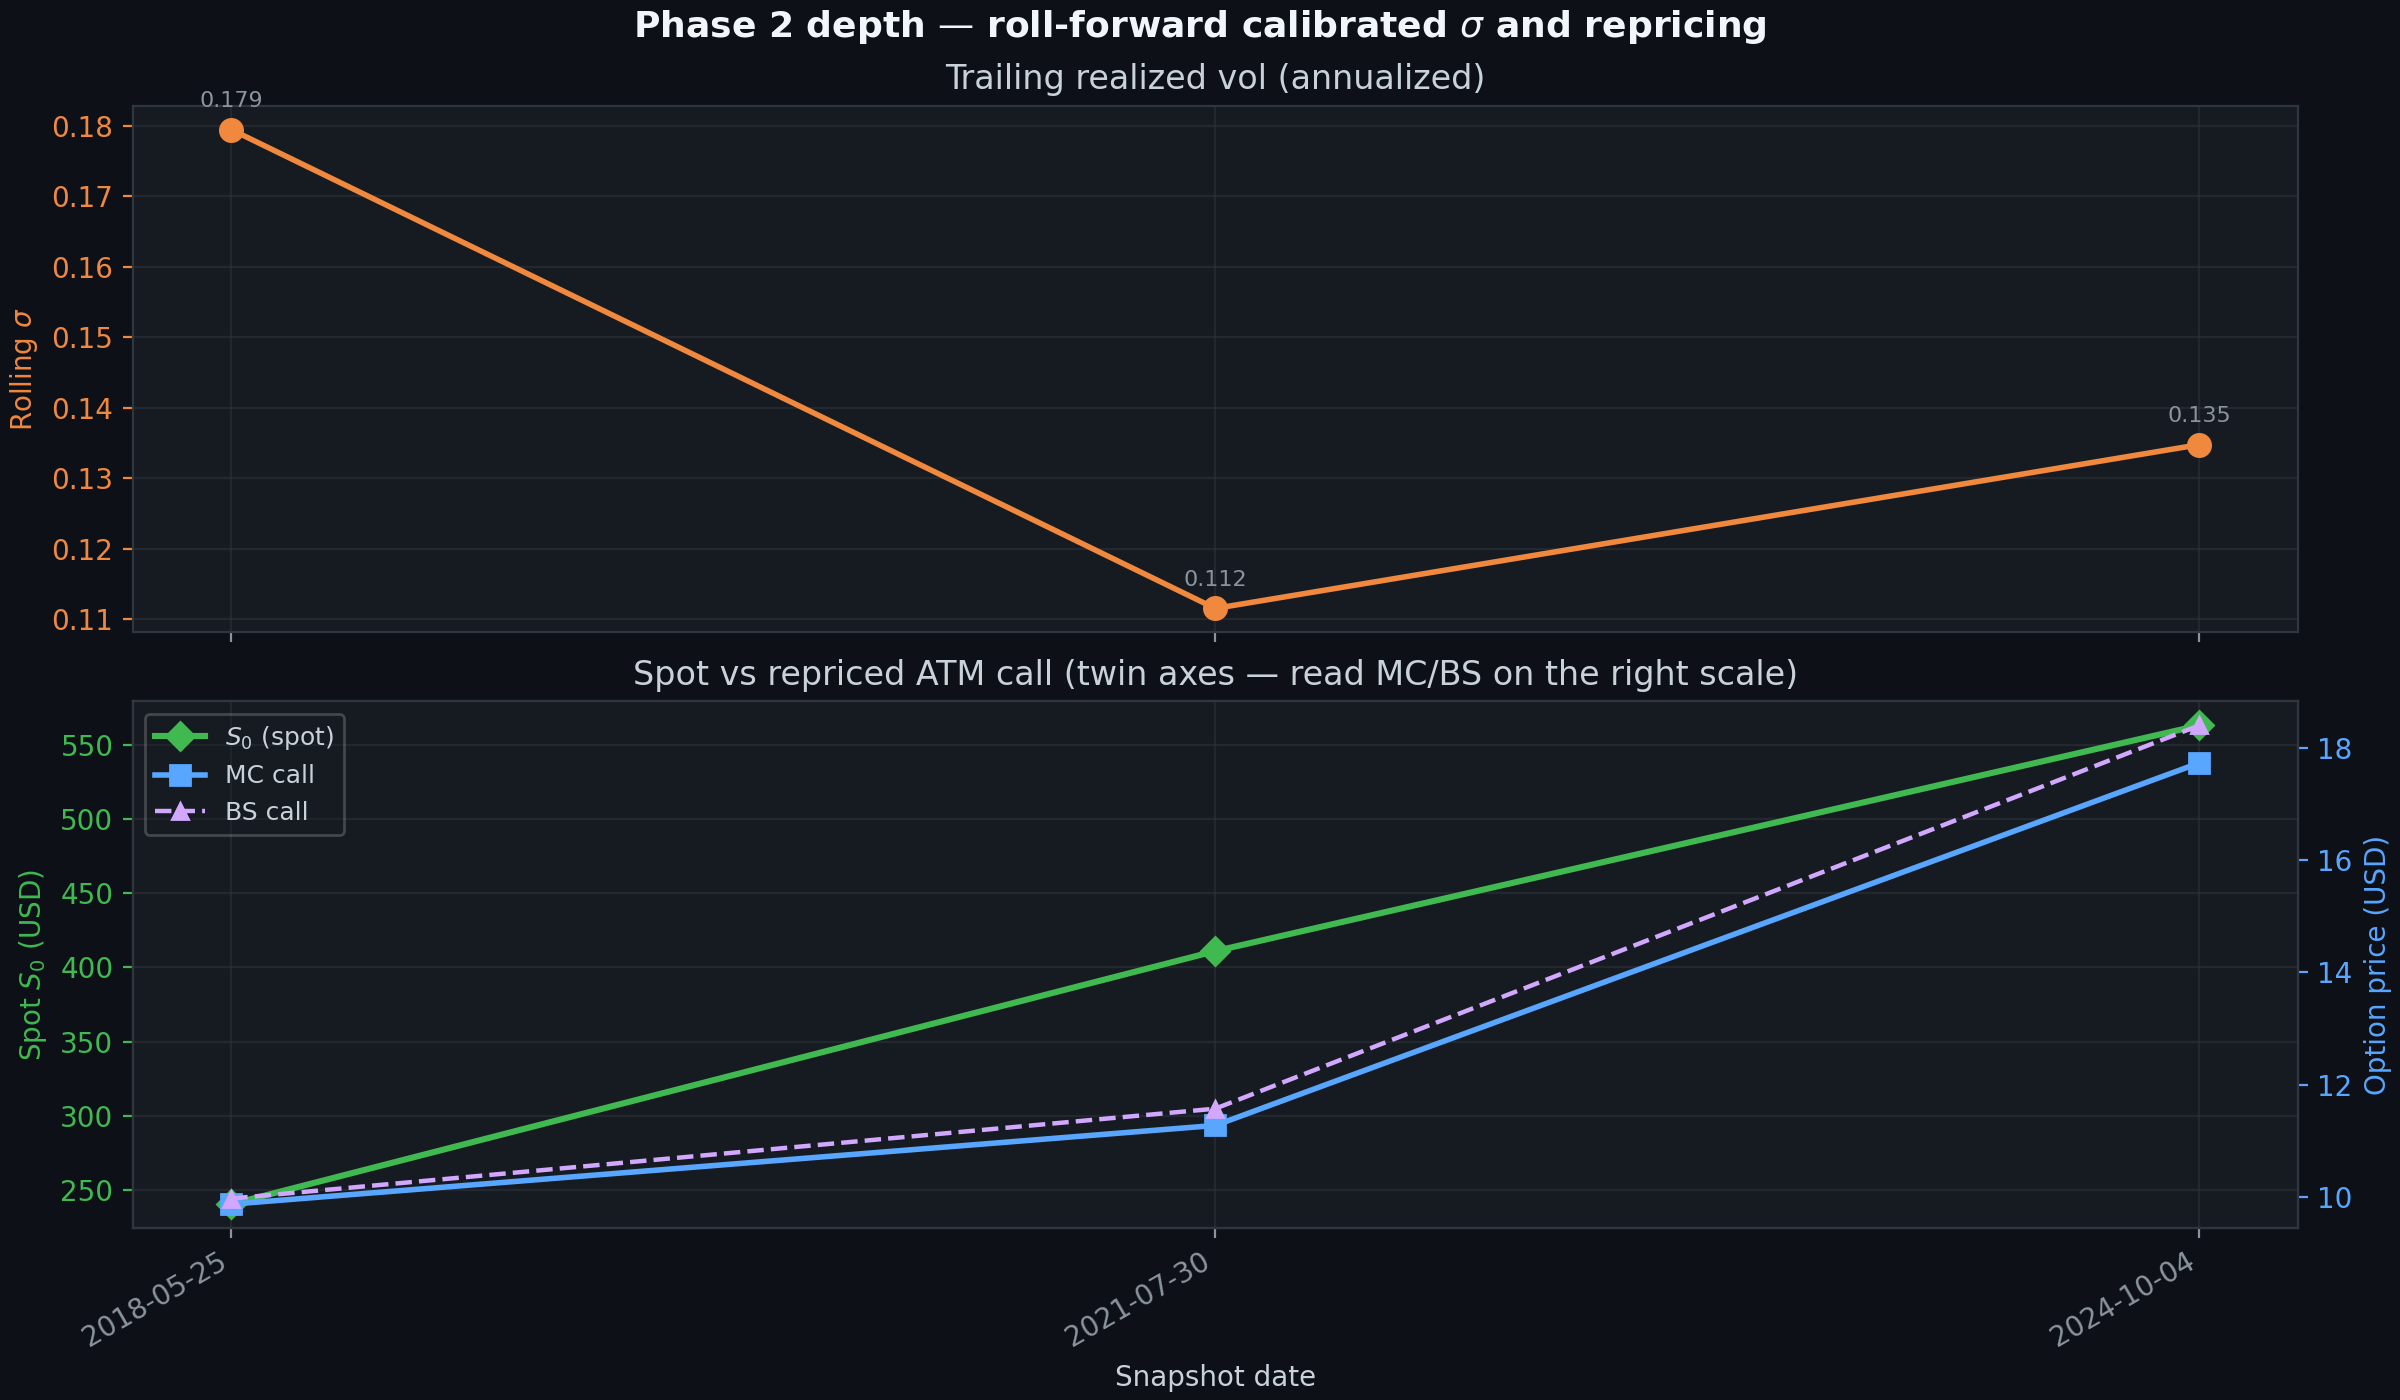
\includegraphics[width=\figw]{phase2_roll_forward_panel.png}
  \caption[Roll-forward panel]{Roll-forward calibrated $\sigma$ and repriced call (twin axes).
  \textbf{Context:} each roll date refreshes the volatility input and re-runs pricing.
  \textbf{Why it matters:} it proves the ``same code, moving inputs'' story for the
  report's Phase~2 claim. \textbf{How to read it:} parallel movements in call value
  and $\sigma$ indicate the dominant sensitivity is vega/vol; divergences would
  point to moneyness or rate effects creeping in through the pricing surface.}
  \label{fig:phase2-roll}
\end{figure}

\section{Figures: Poisson verification, sweeps, and scaling}

\begin{figure}[!h]
  \centering
  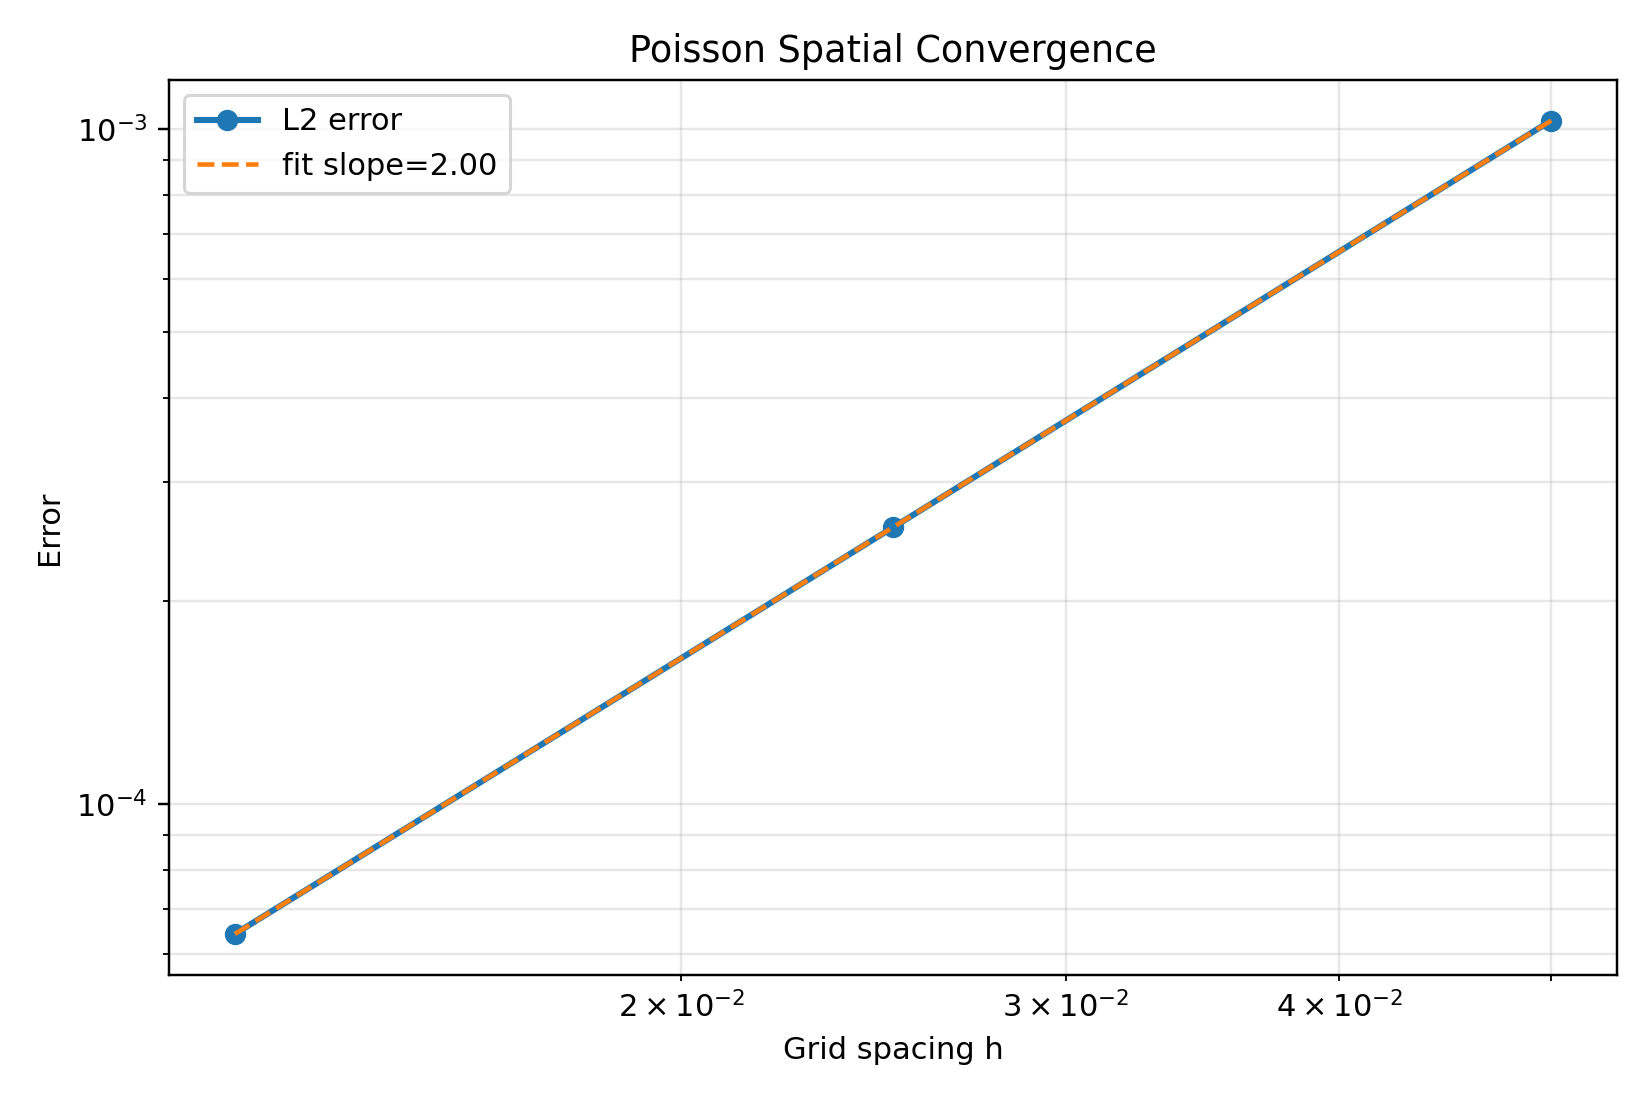
\includegraphics[width=\figw]{spatial_convergence_loglog.png}
  \caption[Poisson spatial convergence]{Poisson $L^2$ error vs.\ mesh spacing on log--log scales.
  \textbf{Context:} this is the deterministic verification anchor for the PETSc FD
  stack. \textbf{Why it matters:} without this plot, solver sweeps are ``moving
  numbers on a broken model.'' \textbf{How to read it:} a line whose slope matches
  the discretization order indicates the implementation matches theory; curvature or
  scatter at the coarsest end often means the asymptotic regime has not been reached.}
  \label{fig:poisson-conv}
\end{figure}

\begin{figure}[!h]
  \centering
  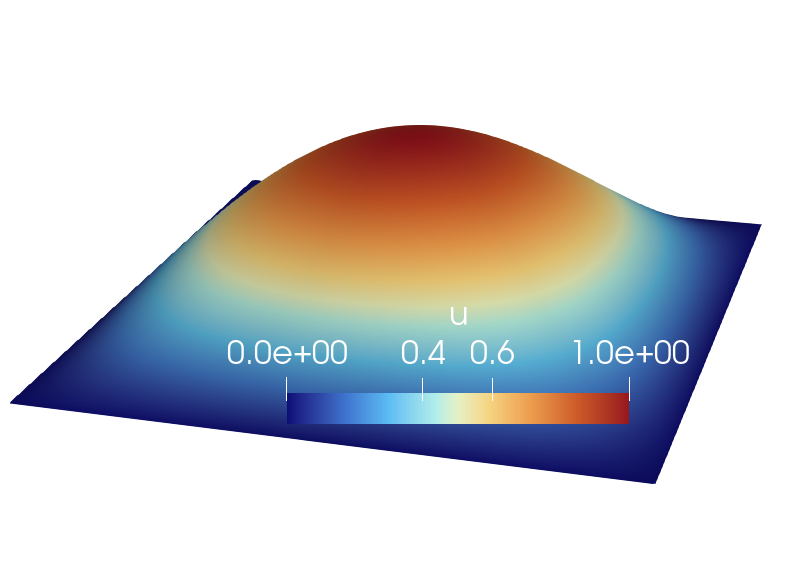
\includegraphics[width=\figwp]{poisson_solution_surface.png}\hfill
  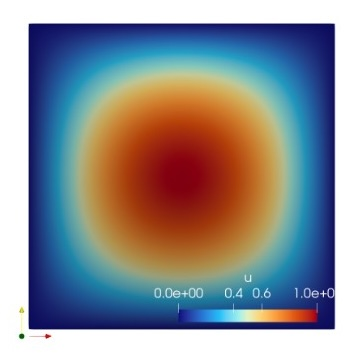
\includegraphics[width=\figwp]{poisson_contour_slice.png}
  \caption[Poisson surface and slice]{Poisson solution surface and contour/slice visualization.
  \textbf{Context:} elliptic solve on the unit square with manufactured forcing.
  \textbf{Why it matters:} it is the ``shape check'' complement to the log--log
  error curve. \textbf{How to read it:} smooth extrema and symmetric contour levels
  indicate a healthy discrete solution; oscillatory or asymmetric patterns would
  hint at assembly bugs, wrong boundary tags, or inadequate resolution.}
  \label{fig:poisson-surf}
\end{figure}

\begin{figure}[!h]
  \centering
  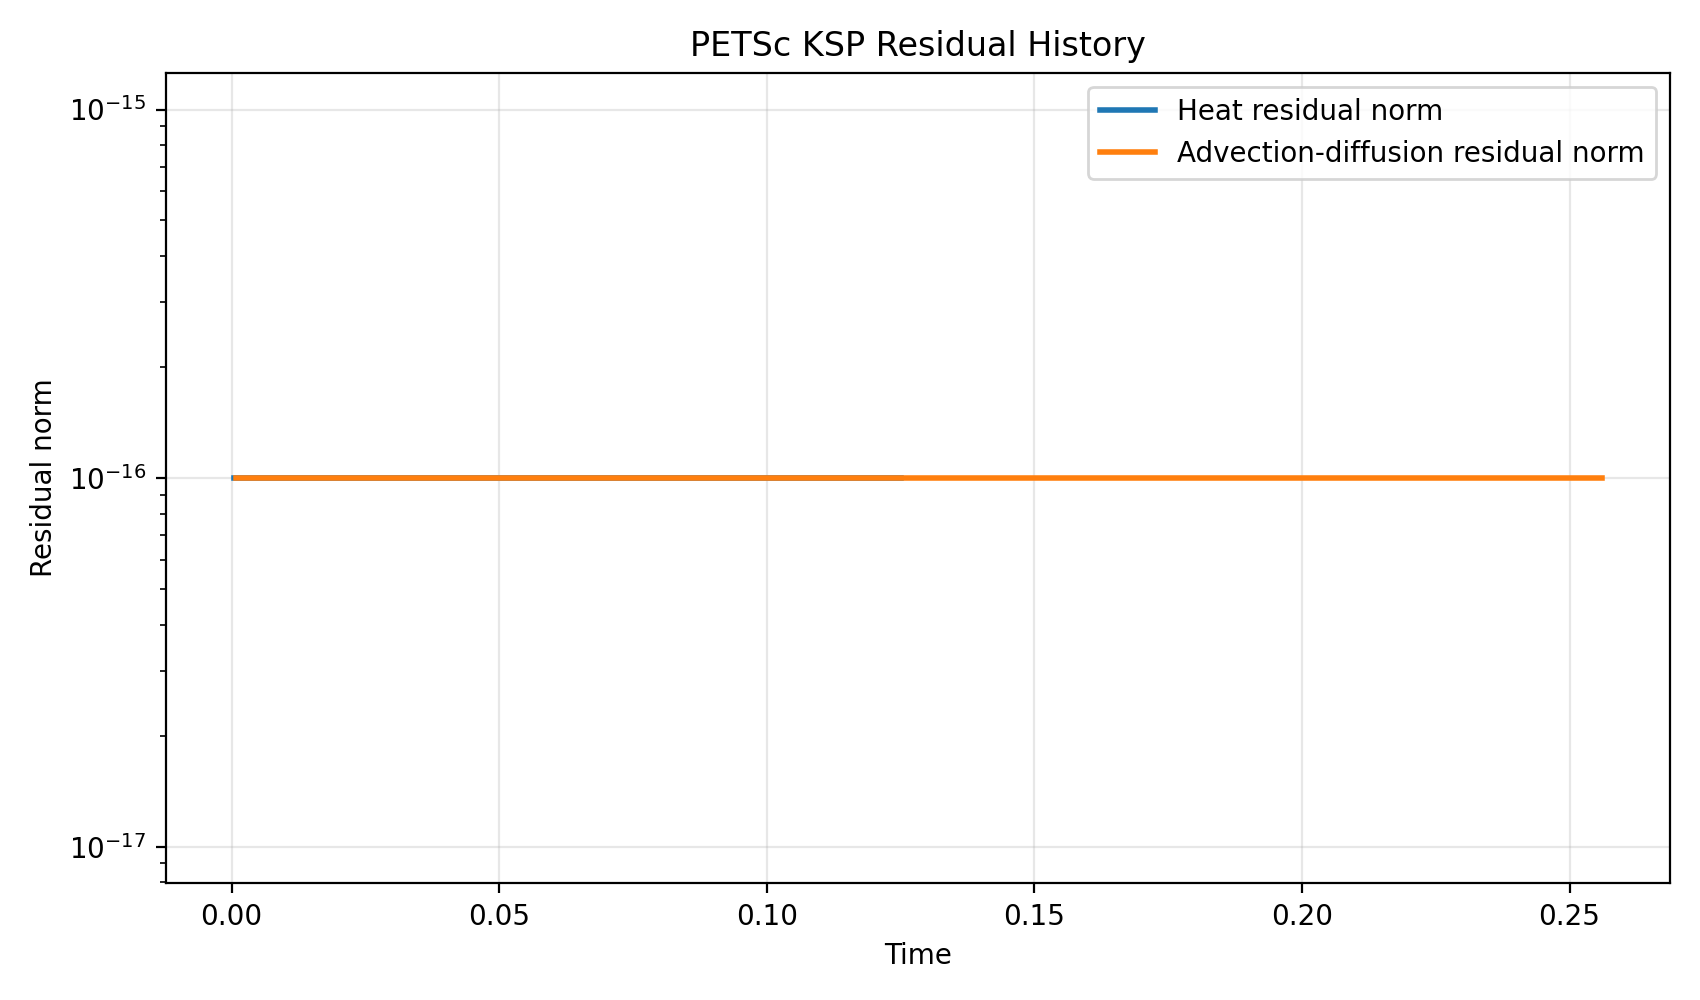
\includegraphics[width=\figw]{poisson_residual_history.png}
  \caption[Poisson residual history]{Representative Poisson residual / solver monitoring figure.
  \textbf{Context:} KSP residual norm vs.\ iteration (or a related diagnostic).
  \textbf{Why it matters:} it documents that the linear solve actually converged and
  how aggressively the preconditioner reduces modes. \textbf{How to read it:} steady
  geometric decay is typical for CG on SPD problems; stagnation or spikes would prompt
  a PC change---matching the sweeps in Figures~\ref{fig:pc-sweep}--\ref{fig:ksp-sweep}.}
  \label{fig:poisson-res}
\end{figure}

\begin{figure}[!h]
  \centering
  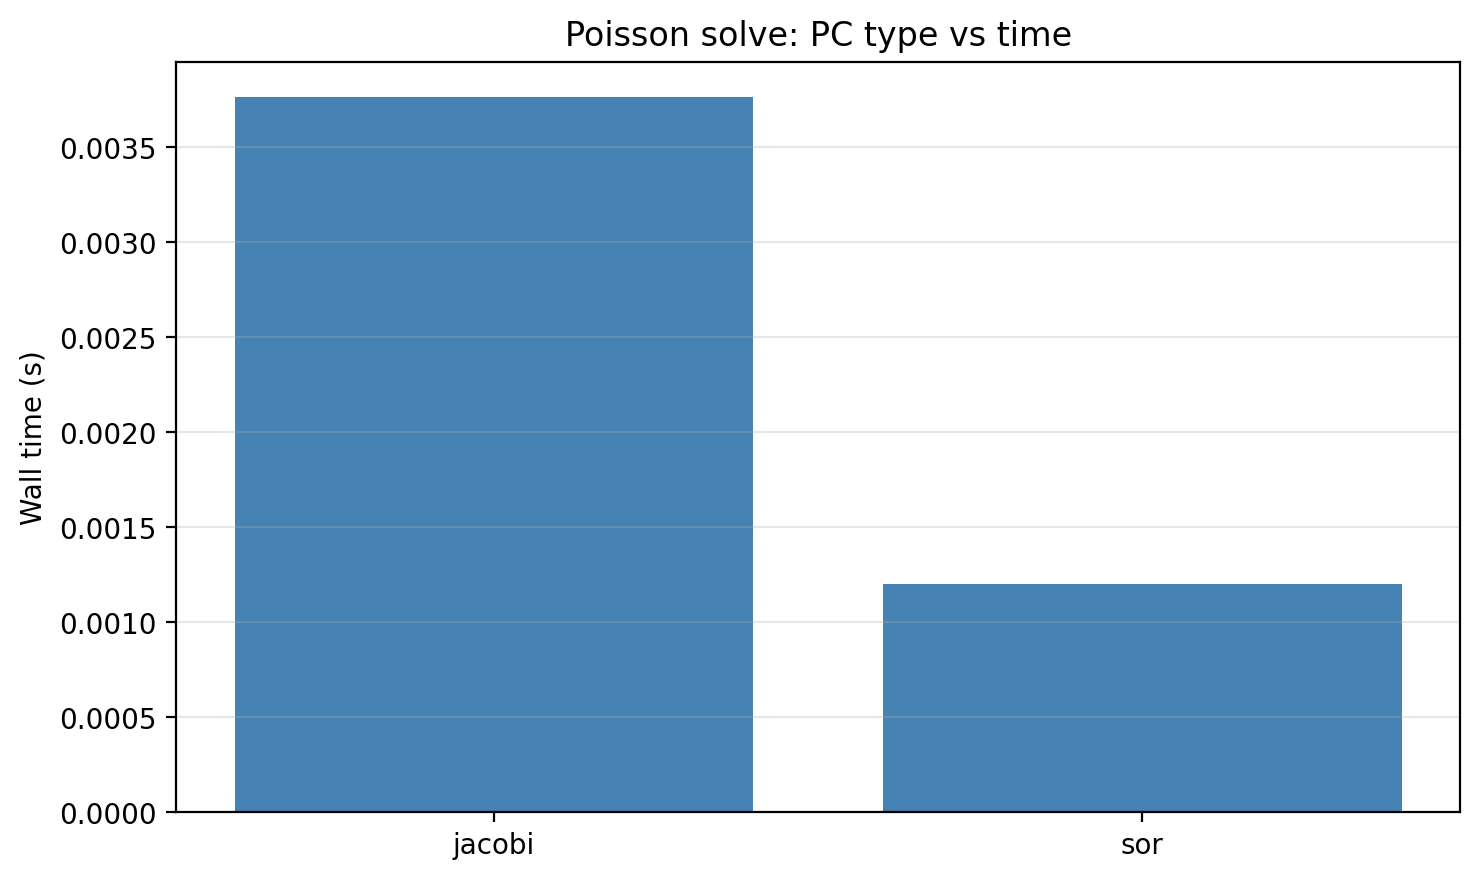
\includegraphics[width=\figwp]{poisson_pc_sweep_time.png}\hfill
  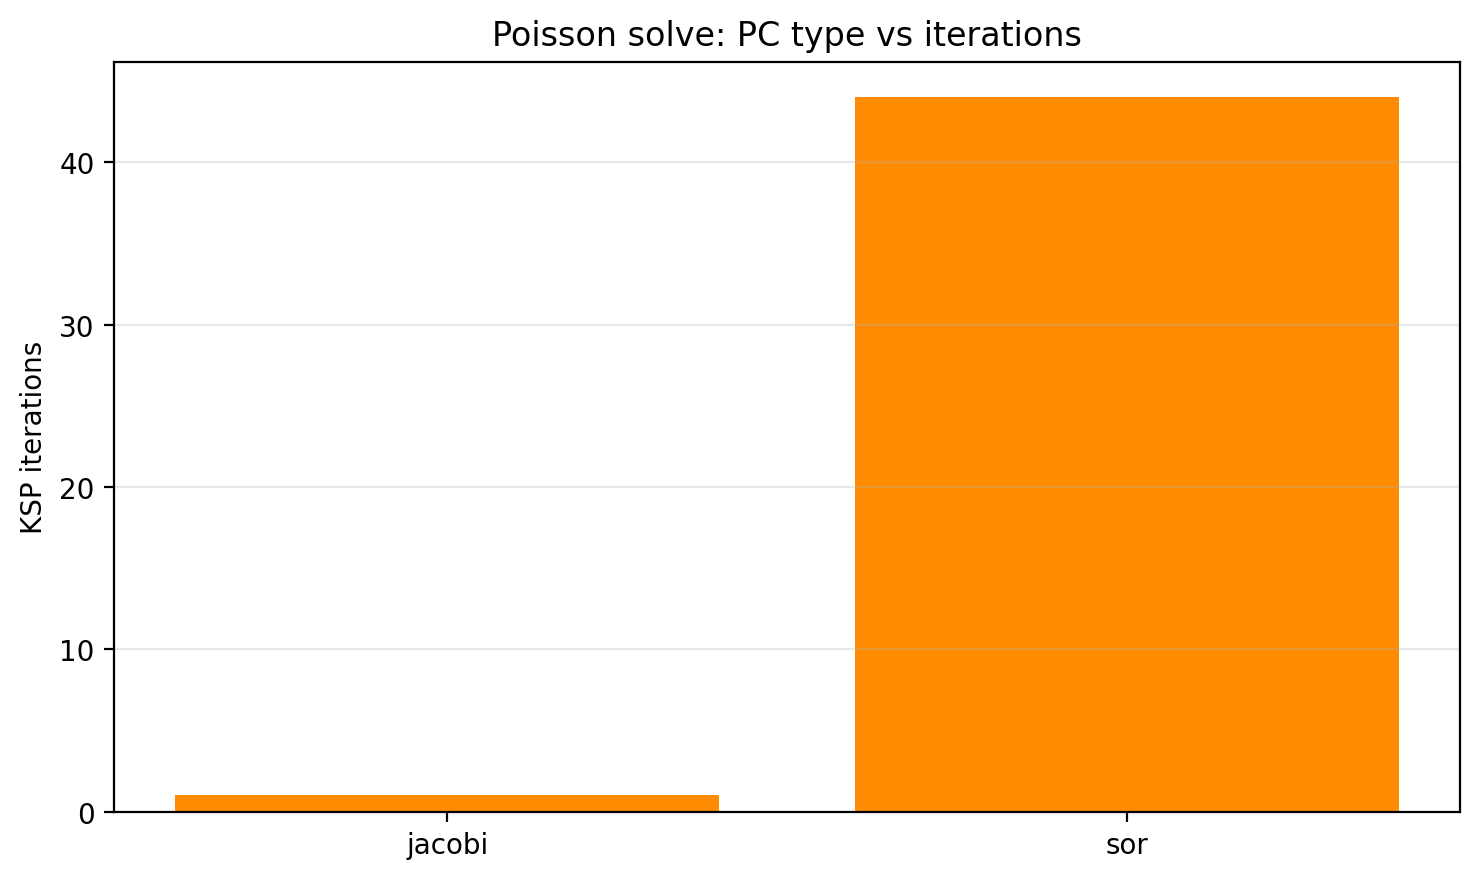
\includegraphics[width=\figwp]{poisson_pc_sweep_iters.png}
  \caption[Poisson PC sweep]{Poisson PC sweep: wall time and iterations vs.\ preconditioner choice.
  \textbf{Context:} controlled experiment on the \emph{same} discrete operator.
  \textbf{Why it matters:} it reinforces that ``parallel PETSc'' is not only about
  ranks---algorithmic preconditioning dominates for ill-conditioned systems.
  \textbf{How to read it:} if time and iterations move together, most cost is Krylov
  work; if time improves while iterations worsen, the preconditioner may be doing
  more expensive local work per step.}
  \label{fig:pc-sweep}
\end{figure}

\begin{figure}[!h]
  \centering
  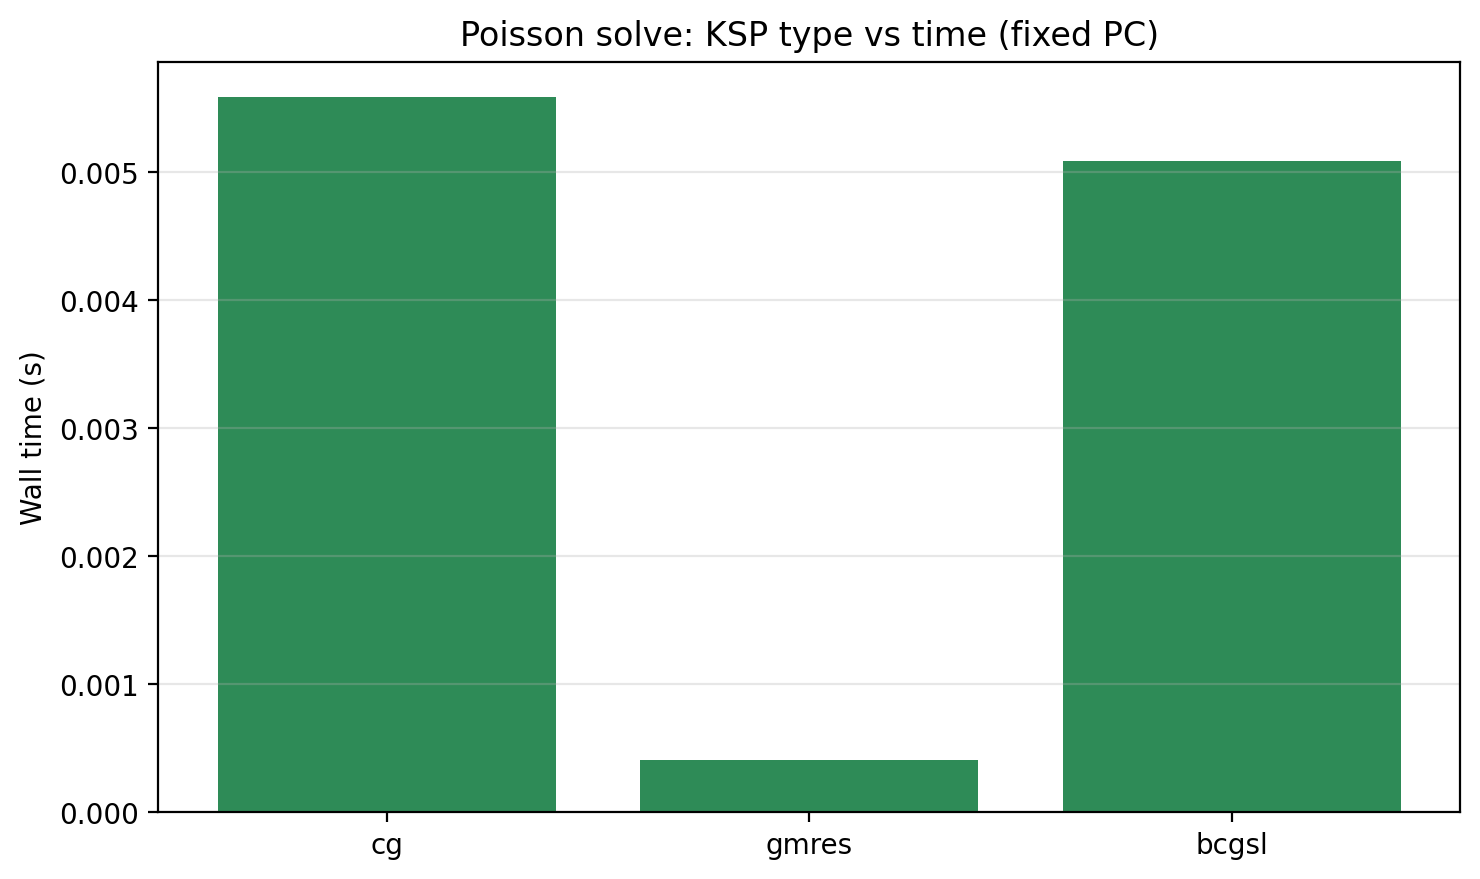
\includegraphics[width=\figwp]{poisson_ksp_sweep_time.png}\hfill
  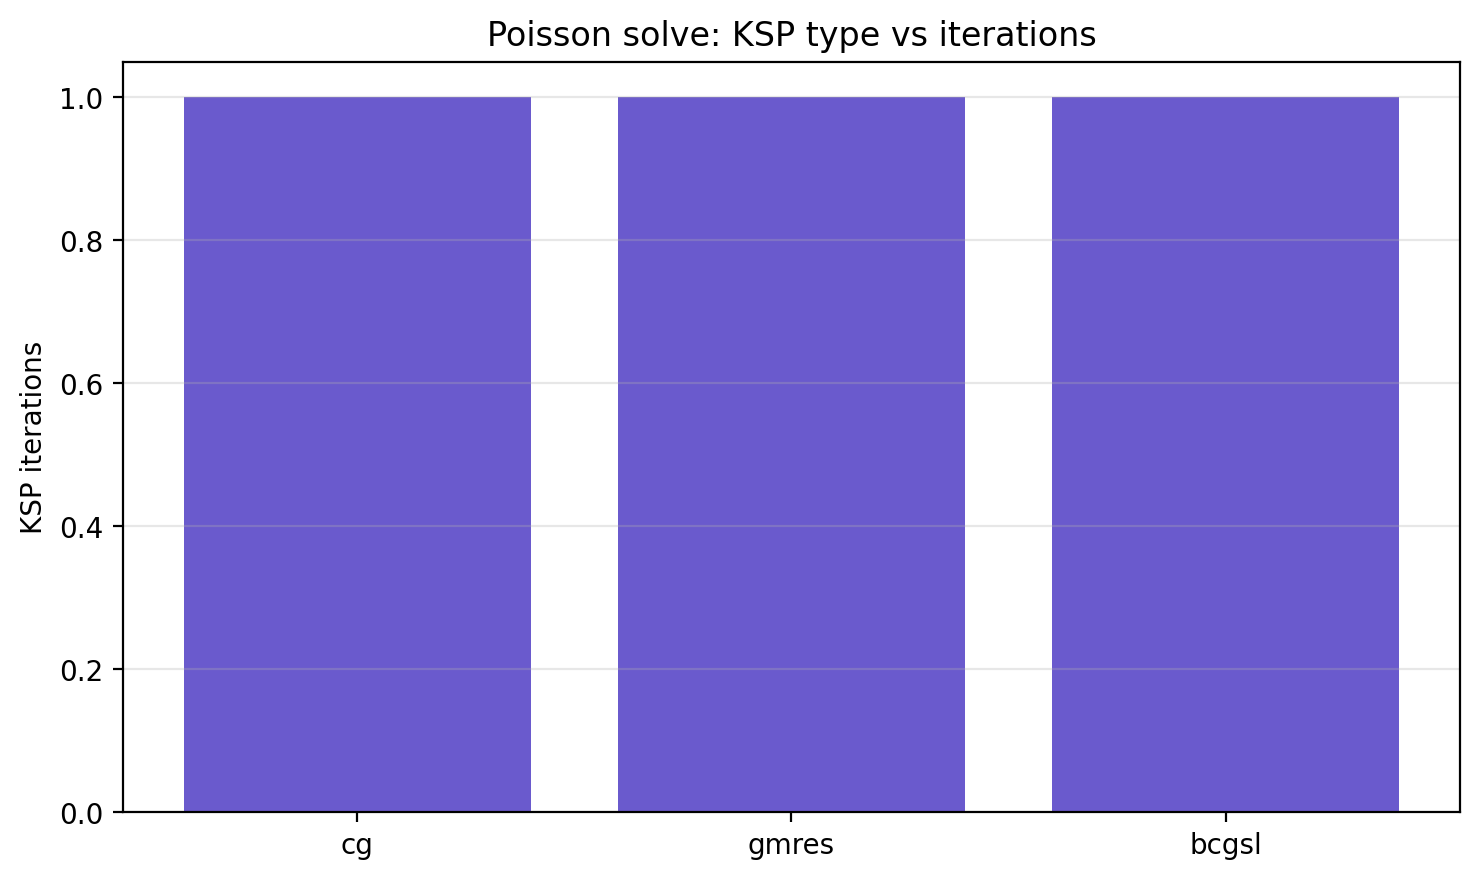
\includegraphics[width=\figwp]{poisson_ksp_sweep_iters.png}
  \caption[Poisson KSP sweep]{Poisson KSP sweep: wall time and iterations vs.\ Krylov method.
  \textbf{Context:} outer solver choice for the same SPD system. \textbf{Why it
  matters:} CG vs.\ GMRES vs.\ other methods differ in memory and stability on
  nonsymmetric extensions. \textbf{How to read it:} on pure Poisson, CG should be
  competitive; large GMRES iteration counts on a nearly SPD problem can signal
  unnecessary nonsymmetric Krylov overhead.}
  \label{fig:ksp-sweep}
\end{figure}

\begin{figure}[!h]
  \centering
  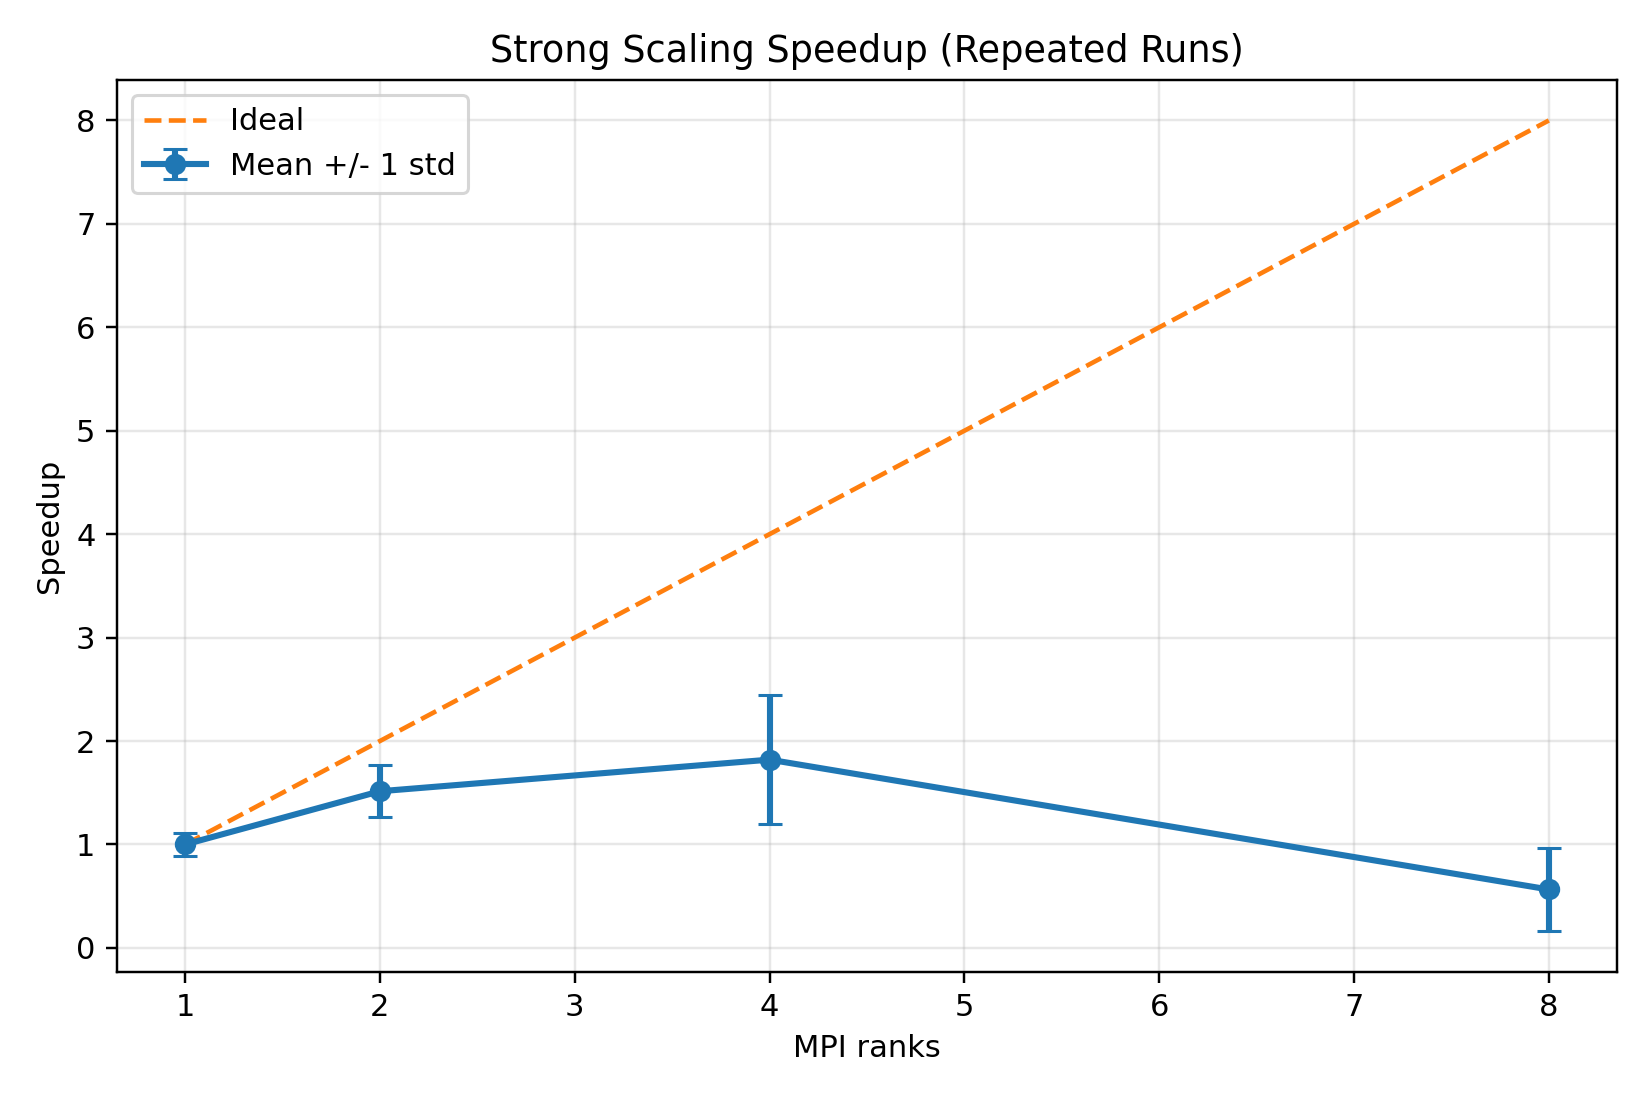
\includegraphics[width=\figw]{strong_scaling_speedup_errorbars.png}
  \caption[Strong scaling speedup]{Poisson strong scaling: speedup with error bars across repeated trials.
  \textbf{Context:} fixed grid, increasing ranks. \textbf{Why it matters:} shows
  whether additional processes reduce wall time in practice. \textbf{How to read it:}
  error bars that overlap the ideal speedup line mean variability is comparable to
  the claimed gain---a common outcome on laptops or shared clusters.}
\end{figure}

\begin{figure}[!h]
  \centering
  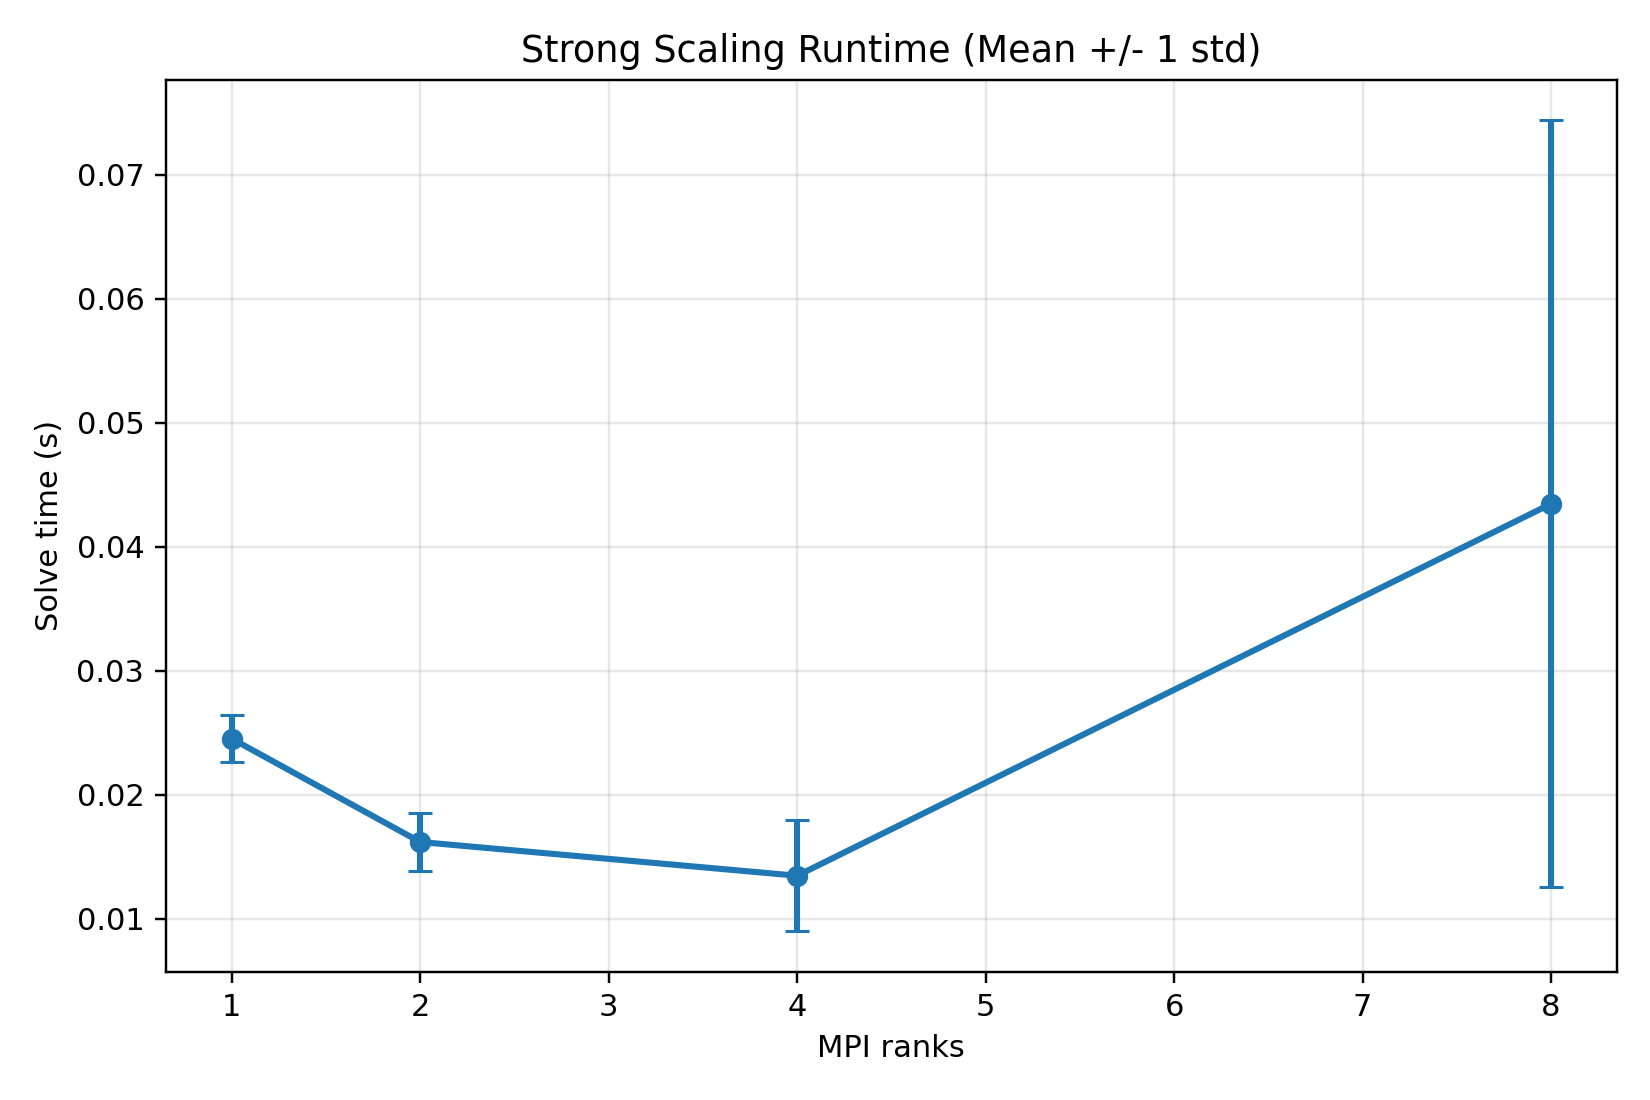
\includegraphics[width=\figw]{strong_scaling_runtime_errorbars.png}
  \caption[Strong scaling runtime]{Poisson strong scaling: runtime variability by rank count.
  \textbf{Context:} complements speedup by showing absolute seconds. \textbf{Why it
  matters:} speedup can look fine while absolute time remains too large for an
  interactive workflow. \textbf{How to read it:} upticks at high rank count often
  mean the problem is too small to amortize communication.}
\end{figure}

\begin{figure}[!h]
  \centering
  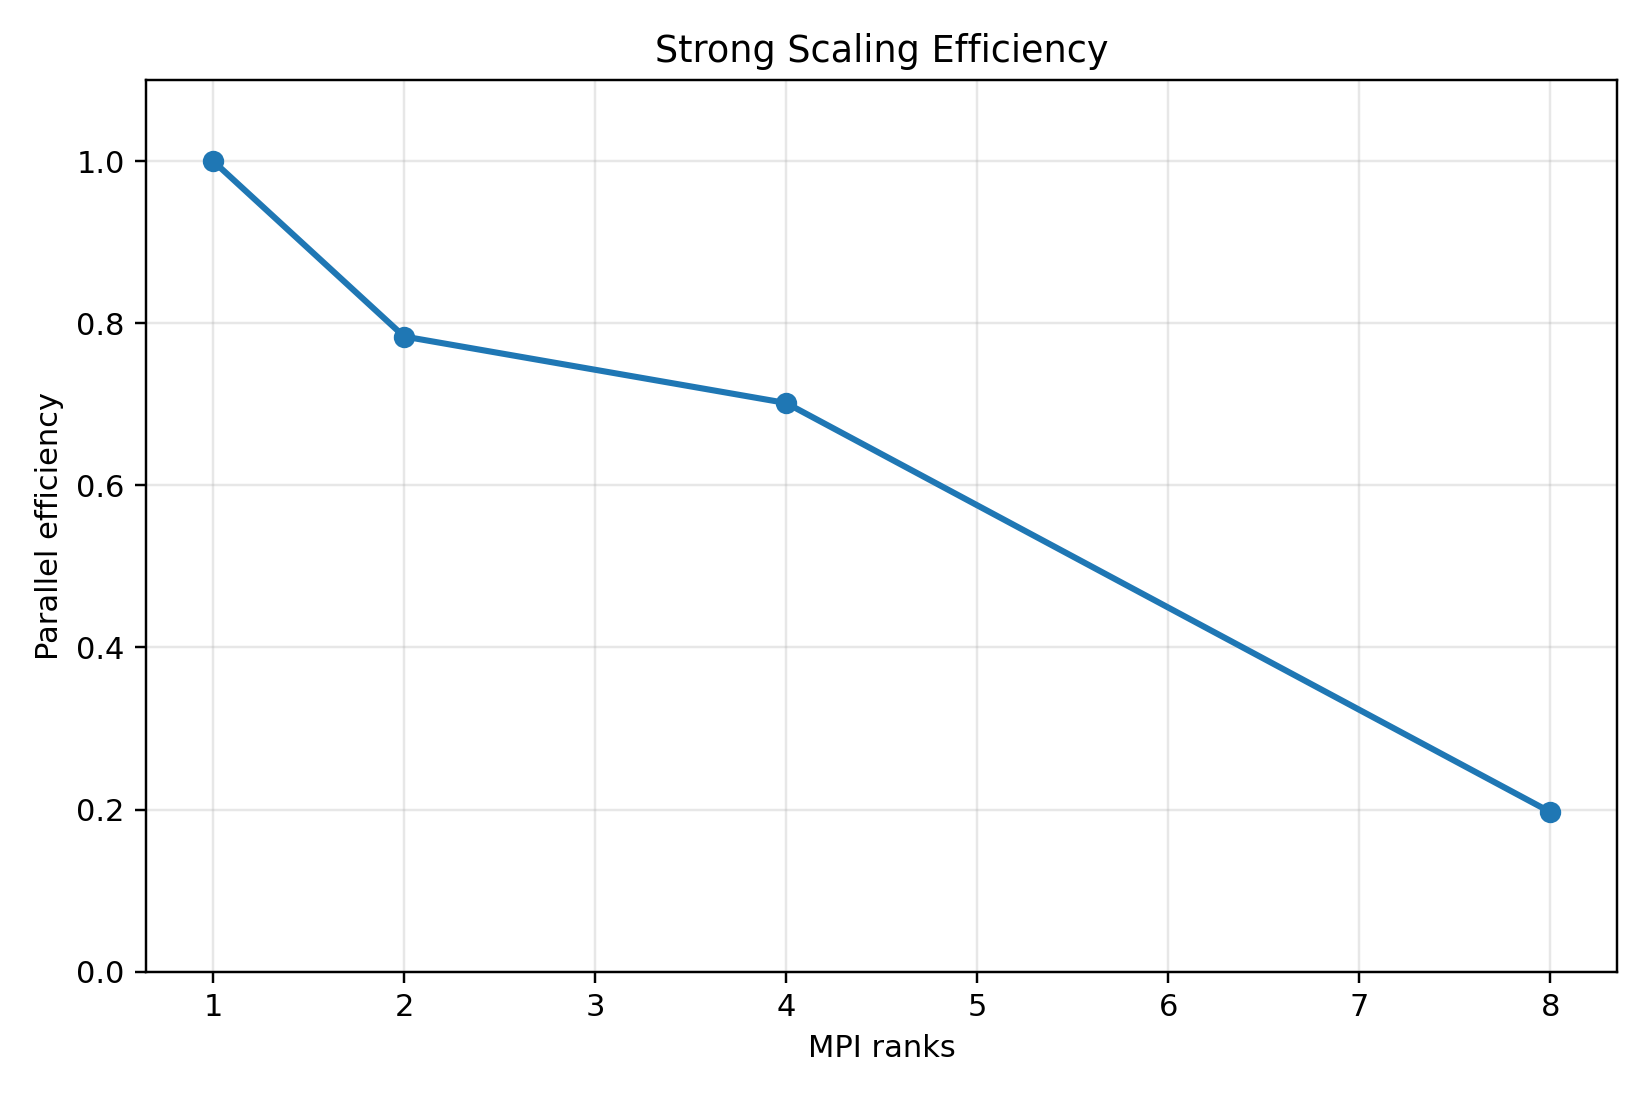
\includegraphics[width=\figw]{strong_scaling_efficiency.png}
  \caption[Strong scaling efficiency]{Poisson strong scaling: parallel efficiency vs.\ ranks.
  \textbf{Context:} efficiency $= \text{speedup}/p$ highlights losses from serial
  fractions and collectives. \textbf{Why it matters:} it is the metric instructors
  often use to temper ``linear speedup'' expectations. \textbf{How to read it:}
  efficiency near one at low $p$ with decline at high $p$ is textbook for a fixed
  small problem; the curve shape matters more than any single point estimate.}
  \label{fig:strong-eff}
\end{figure}

\begin{table}[!h]
  \centering
  \small
  \begin{tabular}{rrrrrr}
    \toprule
    Ranks & Count & Mean time (s) & Std (s) & Speedup & Efficiency \\
    \midrule
    1 & 6 & 0.02453 & 0.00188 & 1.00 & 1.00 \\
    2 & 5 & 0.01620 & 0.00237 & 1.51 & 0.76 \\
    4 & 5 & 0.01348 & 0.00448 & 1.82 & 0.45 \\
    8 & 5 & 0.04346 & 0.03091 & 0.56 & 0.07 \\
    \bottomrule
  \end{tabular}
  \caption{Example Poisson strong-scaling summary (repository snapshot): counts record
  independent timing trials; mean and std summarize variability; speedup uses the
  single-rank mean as baseline; efficiency is speedup divided by ranks. A row where
  speedup drops below one is a faithful record that \textbf{more ranks hurt} for that
  fixed problem size on that machine---not a plotting bug.}
\end{table}

\section{Research conclusions (what we learned)}
\subsection{Monte Carlo conclusions}
The Monte Carlo stack is \textbf{correct in expectation} (European vs.\ BS), shows
\textbf{statistical convergence} consistent with $O(N^{-1/2})$ error decay, and
exhibits \textbf{payoff-driven variance} in barrier regimes. Parallel scaling is
\textbf{empirical}: it summarizes this implementation on this hardware and should be
quoted with that caveat.

\subsection{PDE / Krylov conclusions}
Poisson mesh refinement provides the deterministic credibility layer. Solver sweeps
support the broader lesson from Bueler~\cite{bueler2020petsc} and PETSc
documentation~\cite{petsc-user-ref}: \textbf{algorithmic choices matter as much as
``big-$N$ parallelism''} for wall time and iteration counts.

\subsection{Phase~2 conclusions}
Realized volatility is time-varying and event-sensitive; roll-forward repricing
shows that \textbf{identical MC machinery} yields different economic outputs when
inputs are disciplined by data rather than by stylized constants.

\subsection{Next steps: low-hanging fruit}
\label{sec:remaining}
The items below are the easiest wins after freezing the current results---mixing
submission polish with extensions that reuse existing scripts rather than new
theory:
\begin{itemize}[leftmargin=*]
  \item \textbf{Figure sync:} refresh \texttt{overleaf/figures/} from \texttt{visuals/}
  and \texttt{output/} after any re-render (see \texttt{README\_COMPILE.md}); ParaView
  stills are already in this PDF but should be recopied if export parameters change.
  \item \textbf{Numbers vs.\ narrative:} align quoted scalars with
  \texttt{RESULTS\_PHASE1.md} and \texttt{output/registry/experiment\_runs.csv}.
  \item \textbf{Reproducibility one-liner:} add \texttt{PETSC\_DIR}, \texttt{PETSC\_ARCH},
  MPI launcher, ranks, and key command lines to an appendix or footnote (many commands
  already live in \texttt{docs/PROJECT\_SUMMARY\_AND\_PETSC\_CHECKLIST.md}).
  \item \textbf{Course-bridge scripts:} run or explicitly defer Vec demo, SNES implied
  vol, and sampling-vs.-solver benchmark; cite outputs or JSON paths if required.
  \item \textbf{Optional quote comparison:} fill \texttt{data/raw/quotes\_template.csv}
  and run \texttt{compare\_mc\_to\_quotes.py} if market-vs.-model comparison is
  expected.
  \item \textbf{Larger scaling sweeps:} repeat Poisson/MC timing trials with error bars
  (weak-scaling PNGs under \texttt{visuals/} are available but not yet in this PDF).
  \item \textbf{Solver / time-integration knobs:} try GAMG or other PCs where available;
  compare TS-based vs.\ backward-Euler stepping on the parabolic drivers.
  \item \textbf{Final compile:} \texttt{pdflatex} twice; check for undefined references
  and missing \texttt{figures/} files.
\end{itemize}

\section{Discussion, limitations, and conclusion}
\subsection{Limitations}
Monte Carlo uncertainty dominates some plots at moderate $N$; barrier estimates can
be noisy without importance sampling. PDE experiments are intentionally
low-dimensional (2D) and are meant as \textbf{methodological demonstrations}, not
production finance or production CFD. Phase~2 uses realized volatility as a simple
historical estimator rather than a full stochastic volatility model.

\subsection{Closing statement}
This project is worthwhile because it forces an integrated narrative: the same
software ecosystem that supports scalable MC also supports the classical PDE and
solver coursework that PETSc was built to serve~\cite{bueler2020petsc,petsc-user-ref}.
The ``good research conclusion'' is not a single number---it is an evidence chain
linking \textbf{verification}, \textbf{statistical scaling}, \textbf{solver
empirics}, and \textbf{data-conditioned inputs}, each interpreted with the correct
reference class and citation lineage.

\paragraph{Software acknowledgment.}
This work relies on PETSc~\cite{petsc-user-ref,petsc-efficient} and \texttt{petsc4py}.

\begin{thebibliography}{99}

\bibitem{bueler2020petsc}
E. Bueler.
\newblock \emph{PETSc for Partial Differential Equations: Numerical Solutions in {C} and {Python}}.
\newblock SIAM, Philadelphia, PA, 2020.

\bibitem{petsc-user-ref}
S. Balay et al.
\newblock PETSc/TAO Users Manual, Revision 3.24.
\newblock Technical Report ANL-21/39, Argonne National Laboratory, 2025.

\bibitem{petsc-efficient}
S. Balay, W.~D. Gropp, L.~Curfman McInnes, and B.~F. Smith.
\newblock Efficient management of parallelism in object oriented numerical software libraries.
\newblock In E. Arge, A.~M. Bruaset, and H.~P. Langtangen, editors,
\emph{Modern Software Tools for Scientific Computing}, pages 163--202. Birkh{\"a}user Boston, 1997.

\bibitem{blackscholes}
F. Black and M. Scholes.
\newblock The pricing of options and corporate liabilities.
\newblock \emph{Journal of Political Economy}, 81(3):637--654, 1973.

\bibitem{merton1973}
R.~C. Merton.
\newblock Theory of rational option pricing.
\newblock \emph{The Bell Journal of Economics and Management Science}, 4(1):141--183, 1973.

\bibitem{paraview-guide}
J. Ahrens, B. Geveci, and C. Law.
\newblock ParaView: An end-user tool for large data visualization.
\newblock In C.~D. Hansen and C.~R. Johnson, editors, \emph{The Visualization Handbook}, chapter~36. Elsevier, 2005.

\end{thebibliography}

\end{document}
